\documentclass{article}
\usepackage{graphicx}
\usepackage{amsmath}
\usepackage{cleveref}
\usepackage{matlab-prettifier}
\usepackage{float}

\title{Optimal HW3}
\author{Walter Livingston}
\date{April 2024}

\begin{document}

\maketitle

Note: All problems are to be sampled at 10 Hz (Ts=0.1) except for problem \#3.\\

\section*{Question I}
Kalman Filter at its best – simulation (actually the Kalman filter is also quite reliable
when we have an excellent model and low noise sensors). Suppose we have a 2 nd
order system that we are regulating about zero (position and velocity) by wrapping an
“optimal” control loop around the system. The new dynamics of the continuous time
system are given by the closed-loop A matrix:
\begin{gather}
    A_{CL} = \begin{bmatrix}
                 0 &    1 \\
                -1 & -1.4
            \end{bmatrix}
\end{gather}
Suppose our measurement is simply position ($C=\begin{bmatrix} 1 & 0 \end{bmatrix}$). There is a white noise
process disturbance (force, $B_w=\begin{bmatrix} 0 \\ 1 \end{bmatrix}$) acting on the controlled system.
\subsection*{Part A}
Simulate the controlled system with the disturbance force ($1\sigma=1$) for 100 seconds at 10Hz sample rate.
\subsection*{Solution}
\begin{figure}[H]
    \centering
    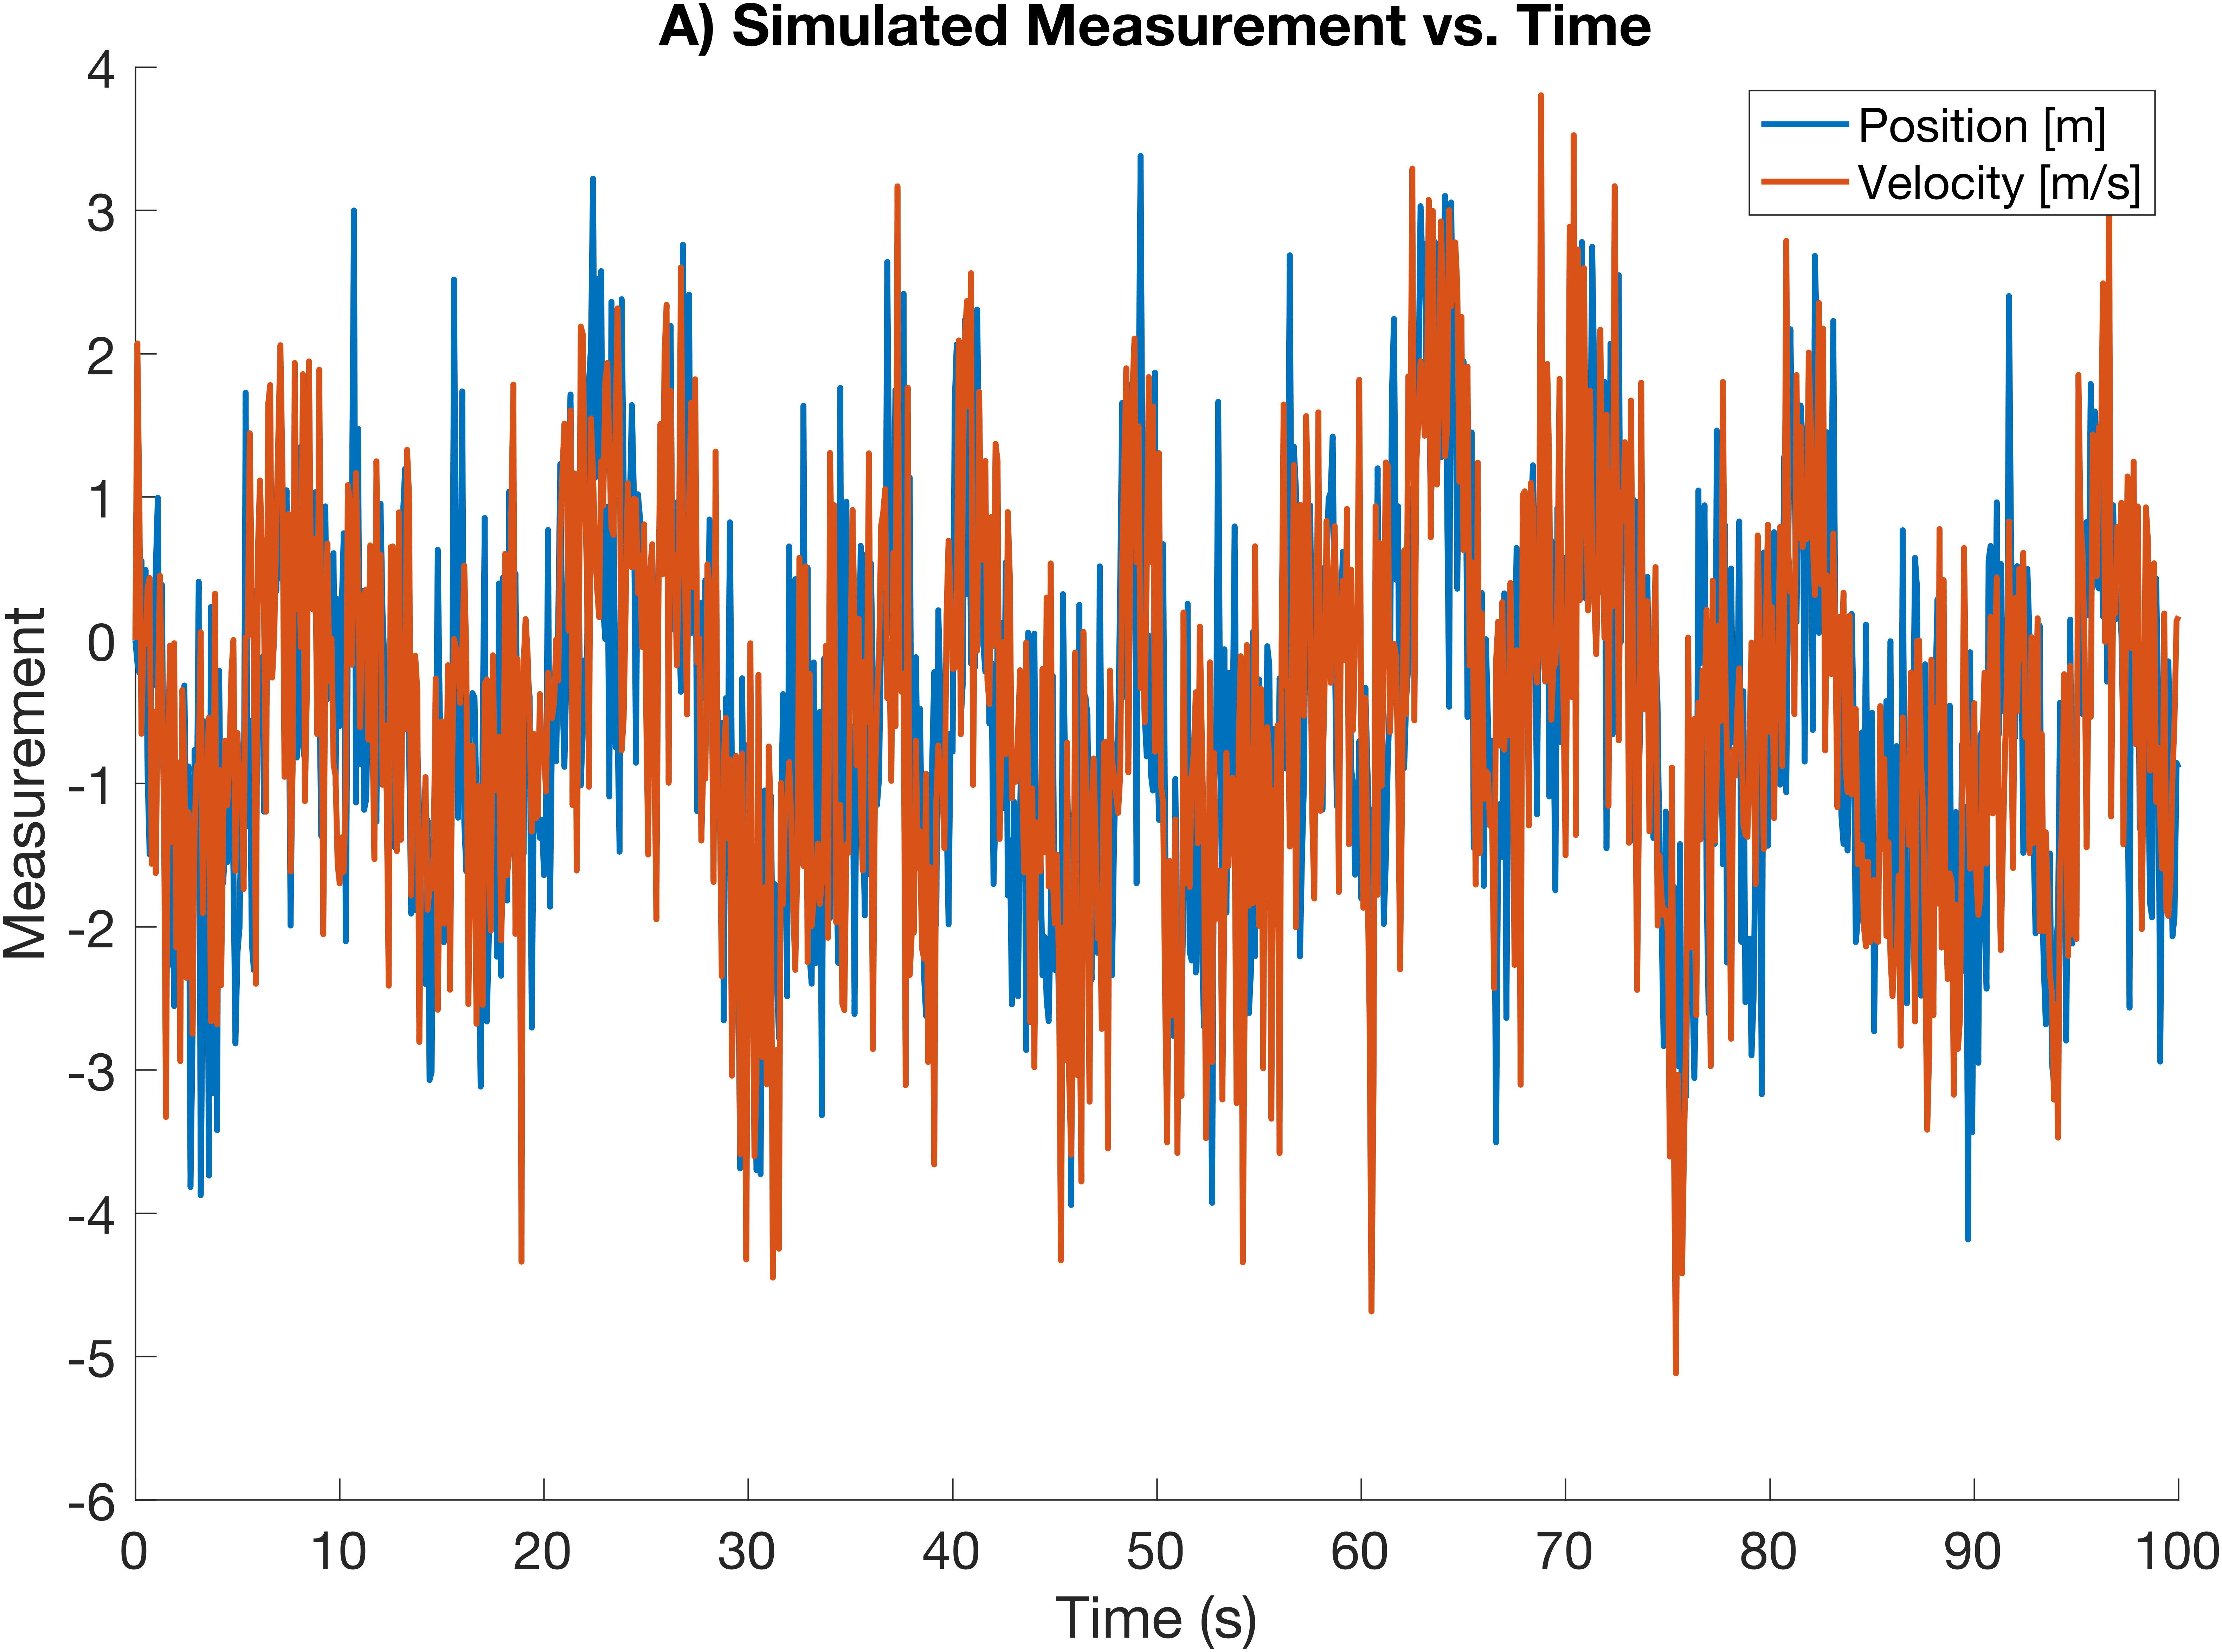
\includegraphics[width=0.75\linewidth]{../figures/p1a.png}
    \caption{Simulated Measurements vs. Time}\label{fig:p1a}
\end{figure}

\subsection*{Part B}
What is $Q, Q_d, R_d$?
\subsection*{Solution}
\begin{gather*}
    Q_c = 4 \\
    Q_d = \int_{}^{}B_w Q_c {B_w}^T d\tau = 0.4\\
    R_d = 1
\end{gather*}

\subsection*{Part C}
Calculate the steady state Kalman gain for the system. This can be done in one of
many ways: iterate the kalman filter until it converges, dlqe.m, dare.m, kalman.m,
dlqr.m (+ predictor to current estimator trick), etc. What is the steady state
covariance of the estimates after the time update, $P^{(-)}$, as well as after the
measurement update, $P^{(+)}$. Where are the poles of the estimator?
\subsection*{Solution}
\begin{figure}[H]
    \centering
    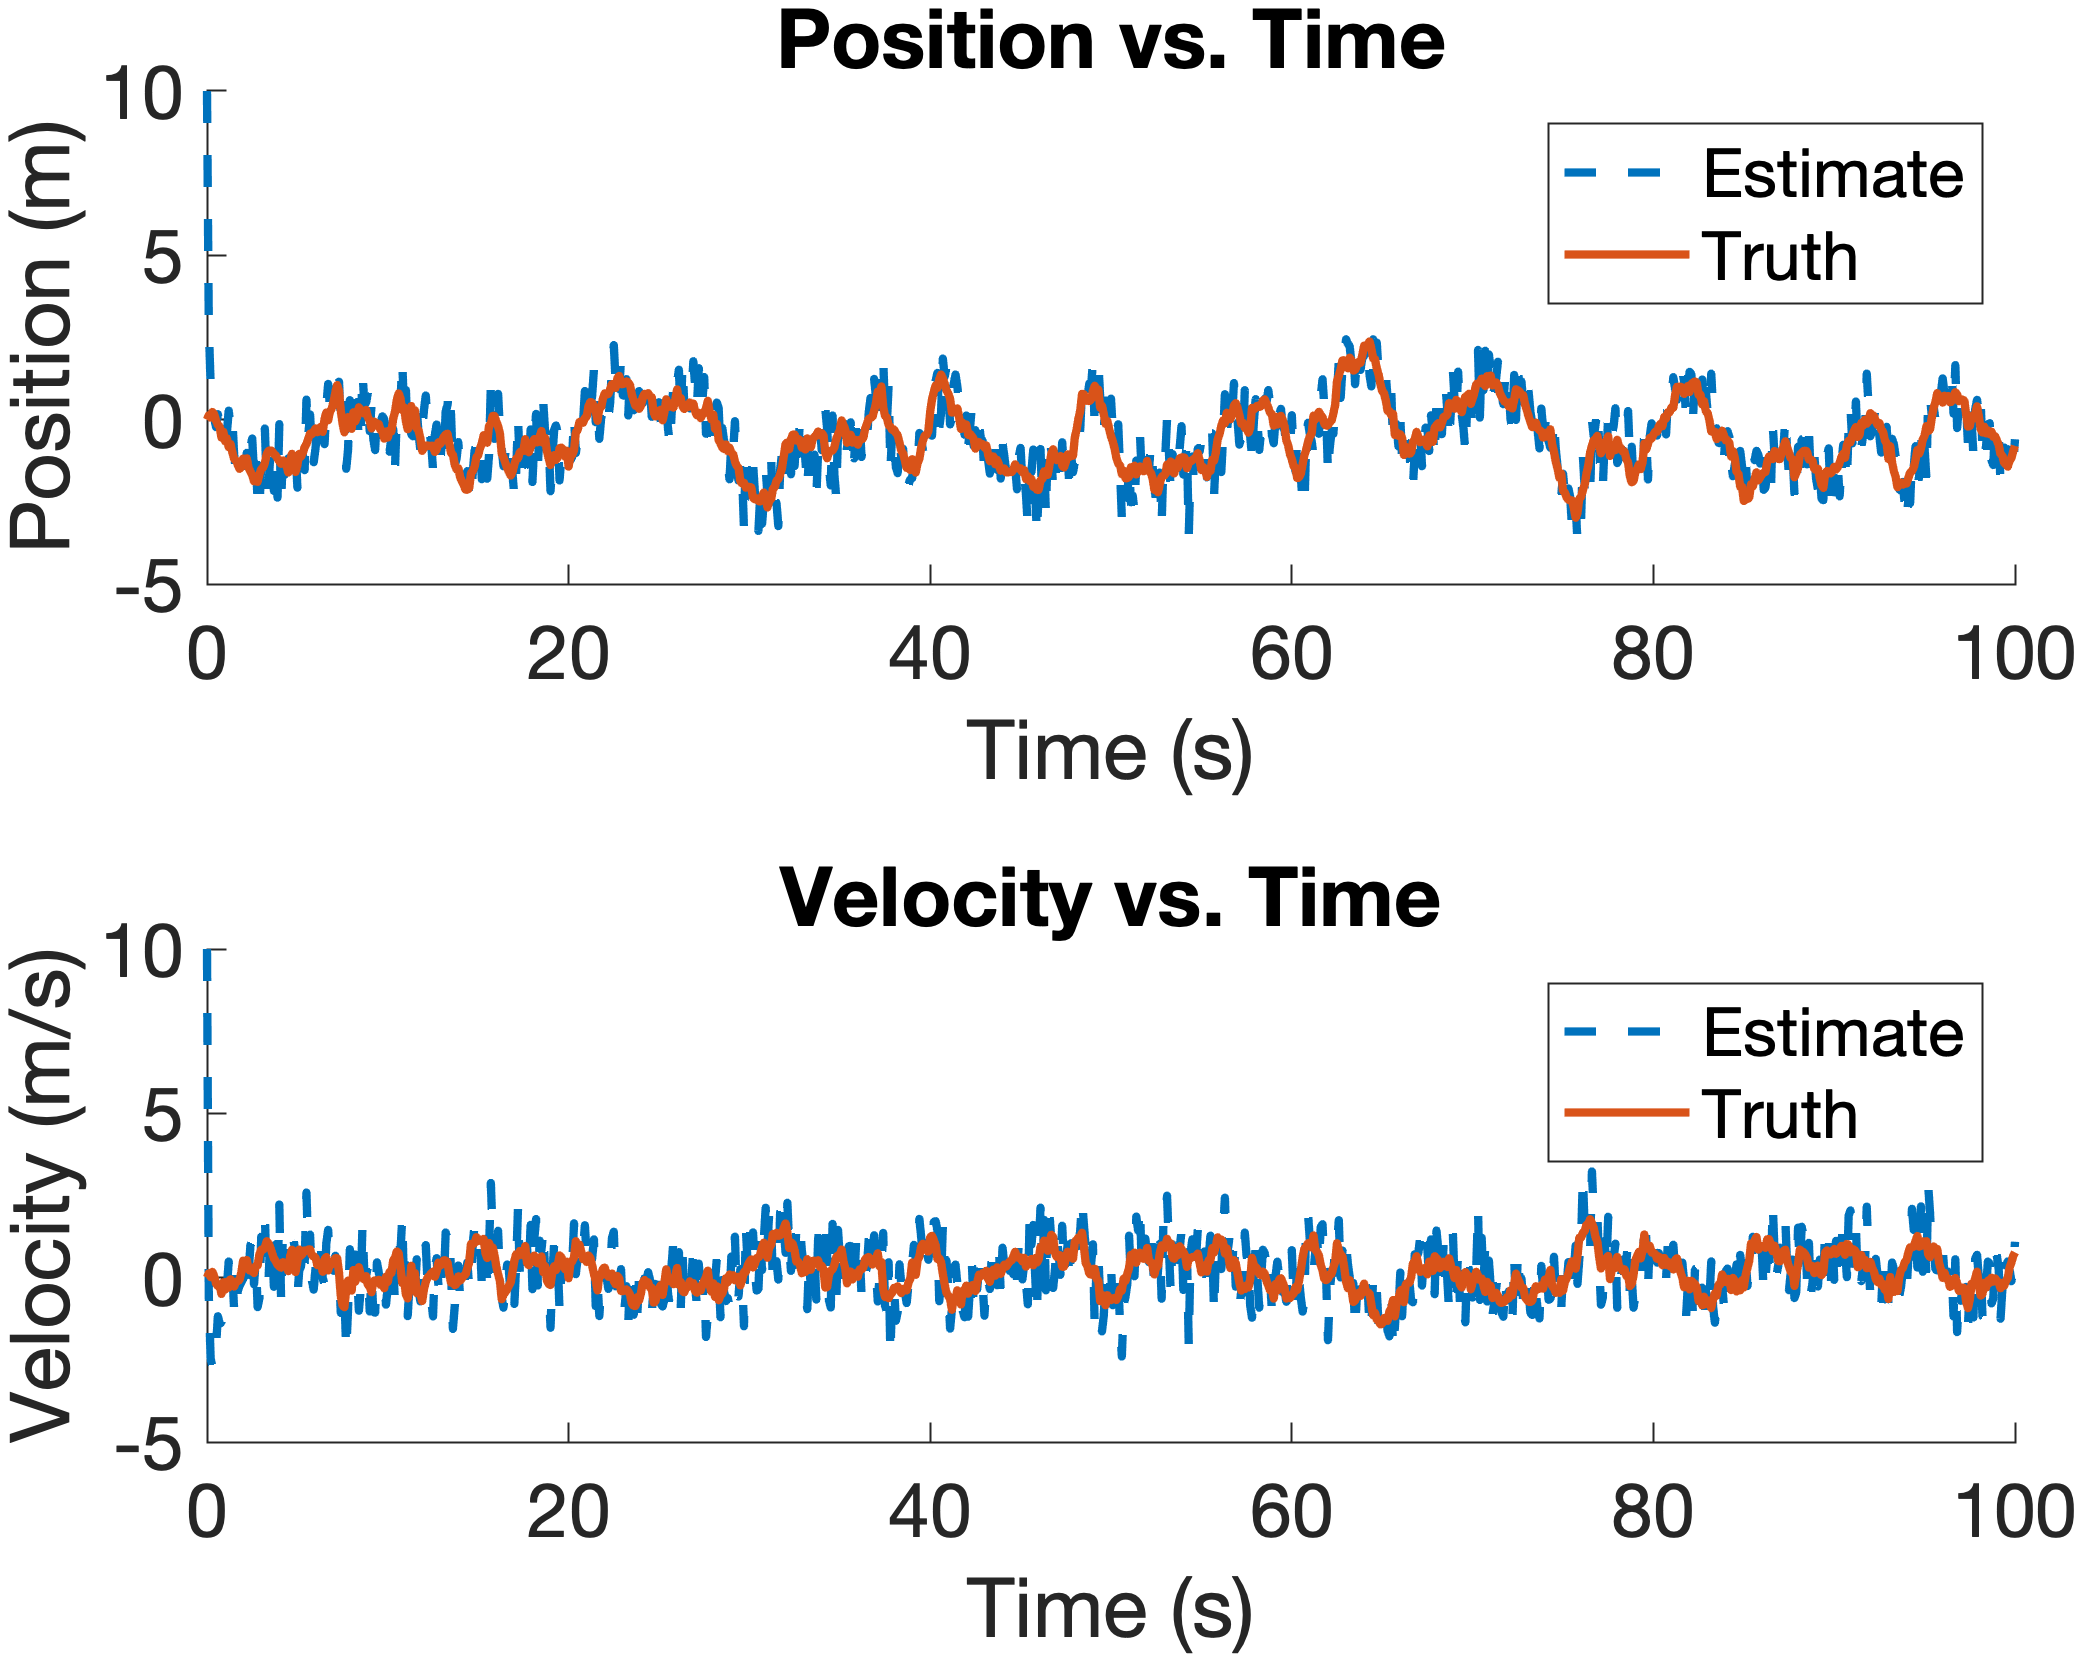
\includegraphics[width=0.75\linewidth]{../figures/p1c1.png}
    \caption{State Estimate vs. Time}\label{fig:p1c1}
\end{figure}

\begin{figure}[H]
    \centering
    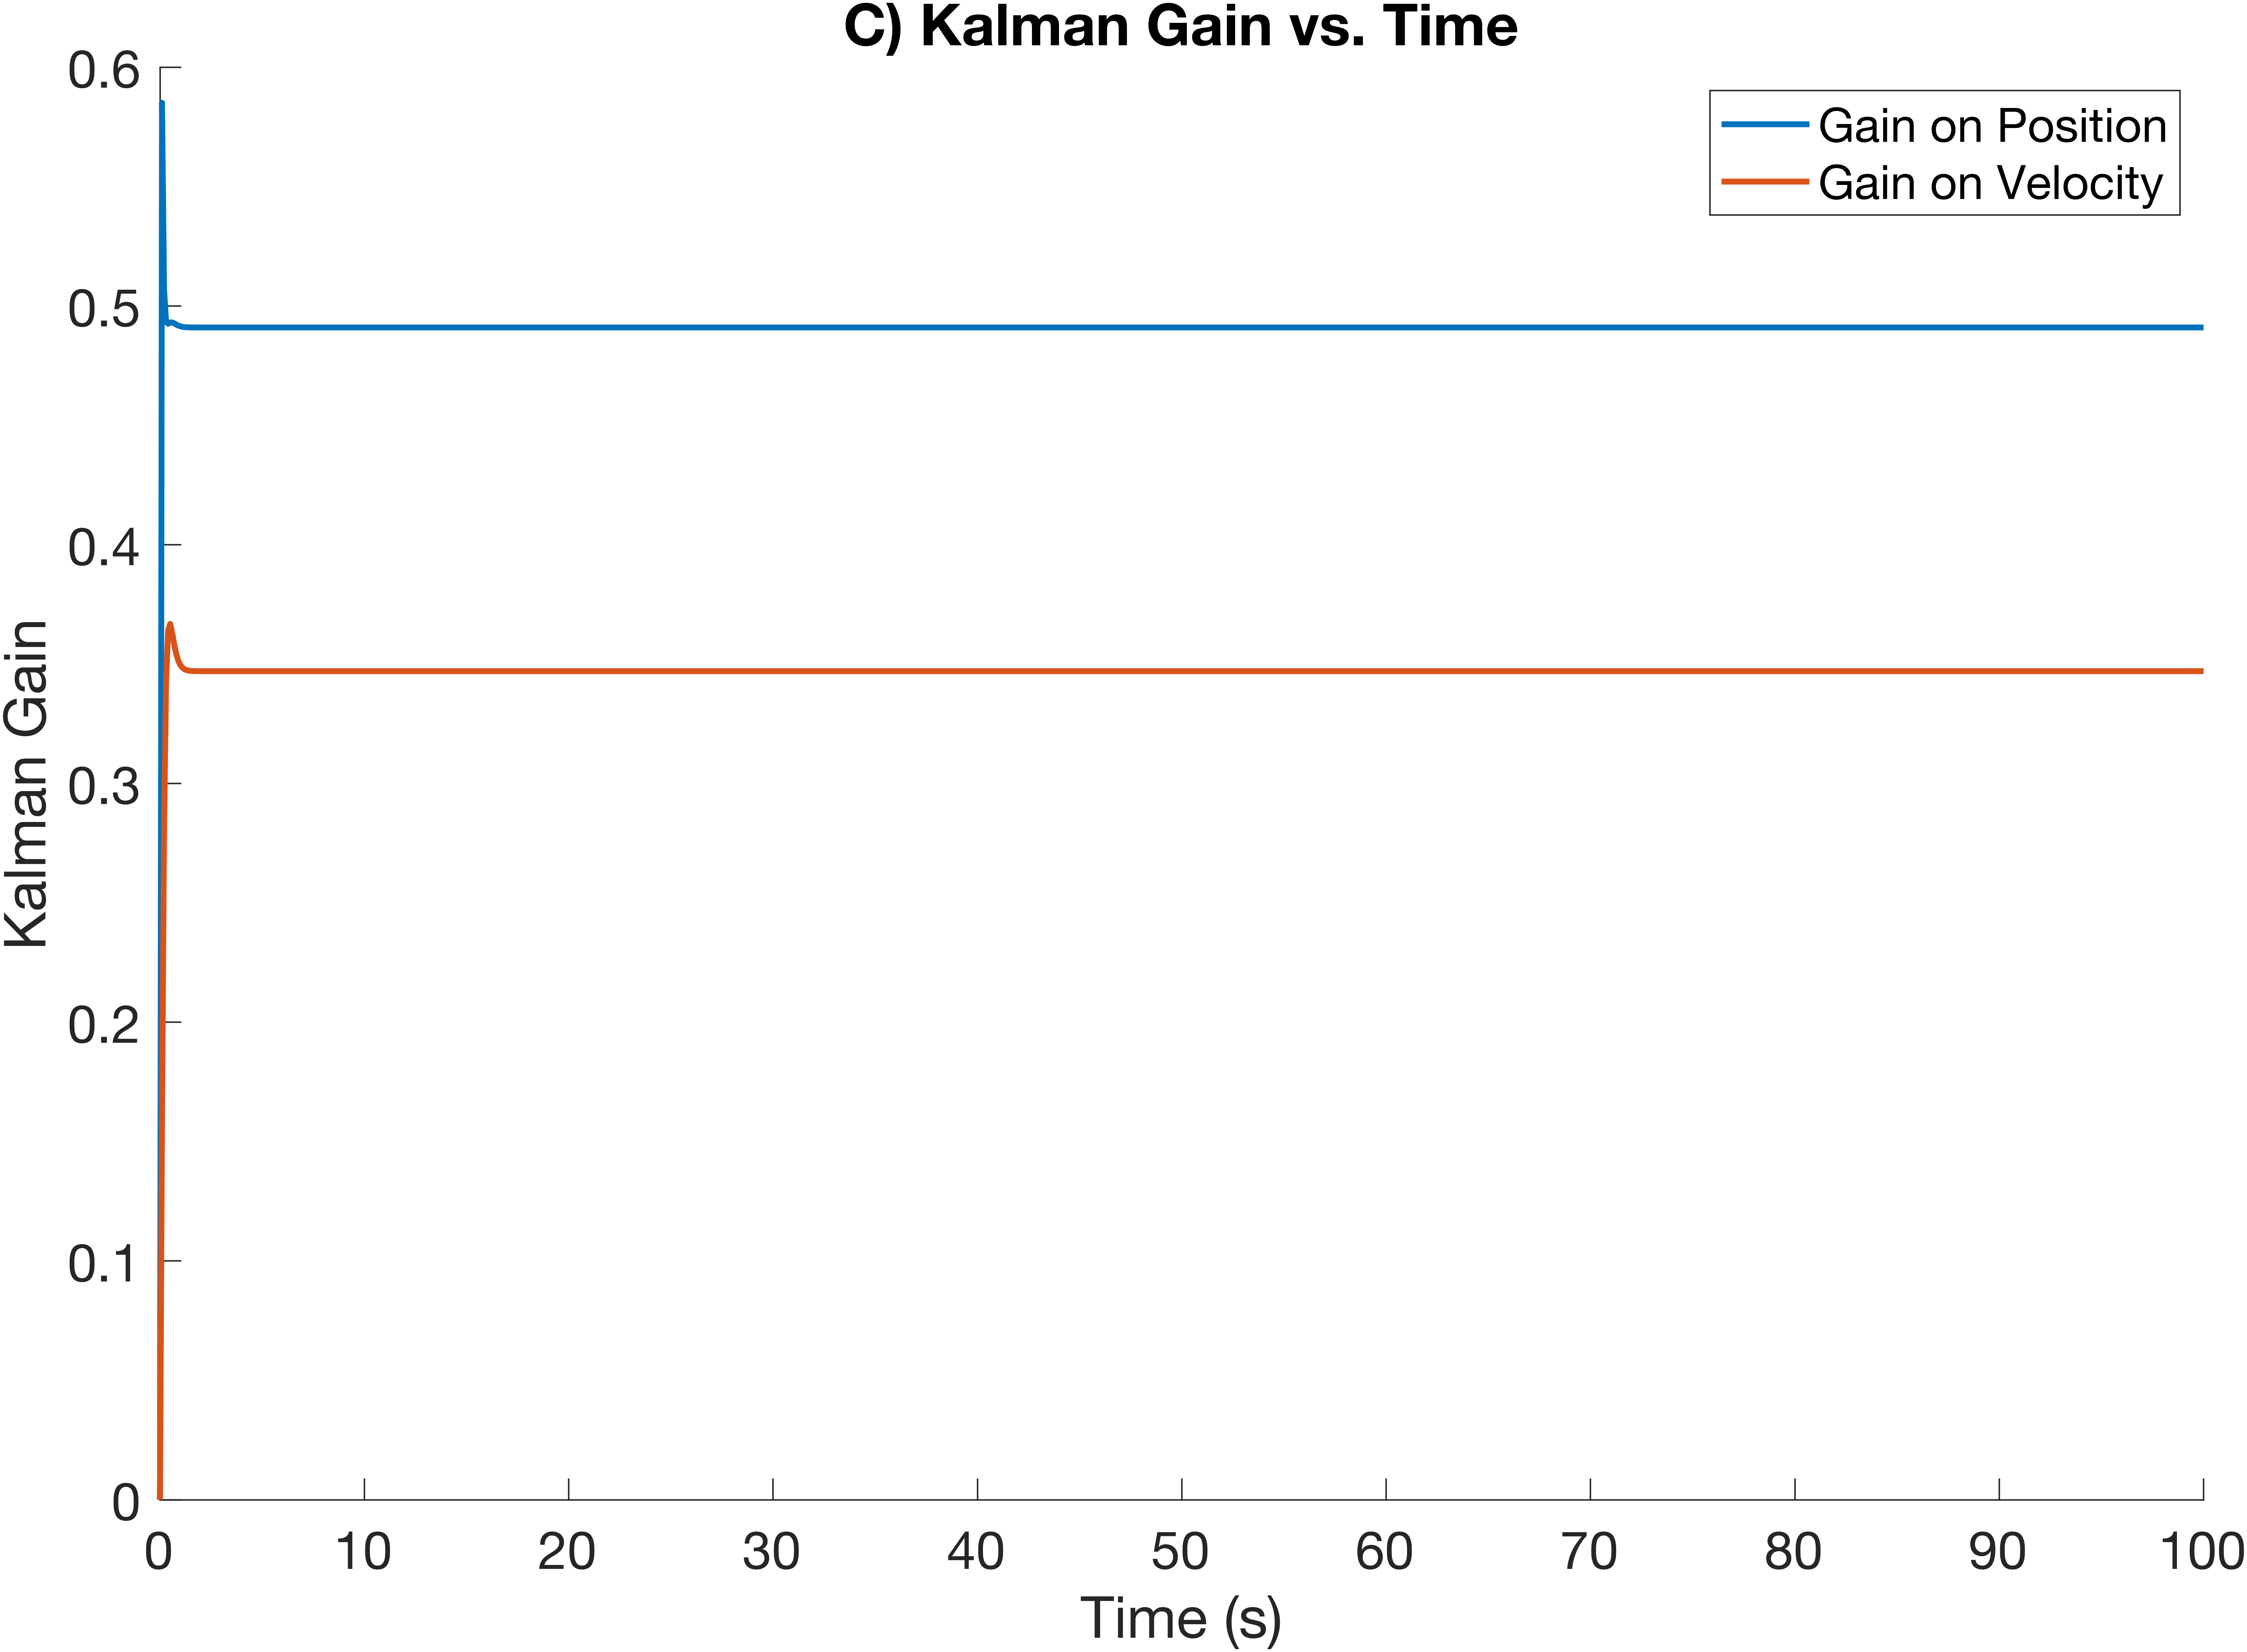
\includegraphics[width=0.75\linewidth]{../figures/p1c2.png}
    \caption{Kalman Gain vs. Time}\label{fig:p1c2}
\end{figure}

\begin{gather*}
    L_{ss} = \begin{bmatrix}
        0.4910\\
        0.3479
    \end{bmatrix}\\
    {P_{ss}}^{-} = \begin{bmatrix}
        0.9646 & 0.6818\\
        0.6818 & 0.6538
    \end{bmatrix}\\
    {P_{ss}}^{+} = \begin{bmatrix}
        0.4910 & 0.3470\\
        0.3470 & 0.4172
    \end{bmatrix}\\
    s = 0.6845 \pm j0.1179
\end{gather*}

\subsection*{Part D}
Now use the steady state kalman filter to generate an estimate ($\hat{x}$ and $\hat{\dot{x}}$) of the 2 states over time.  Calculate the norm of 
the standard deviation of the errors for each state.
\begin{gather}
    N = \sqrt{(std(\dot{x} - \hat{\dot{x}}))^2 + std(x - \hat{x})^2}
\end{gather}
\subsection*{Solution}
\begin{figure}[H]
    \centering
    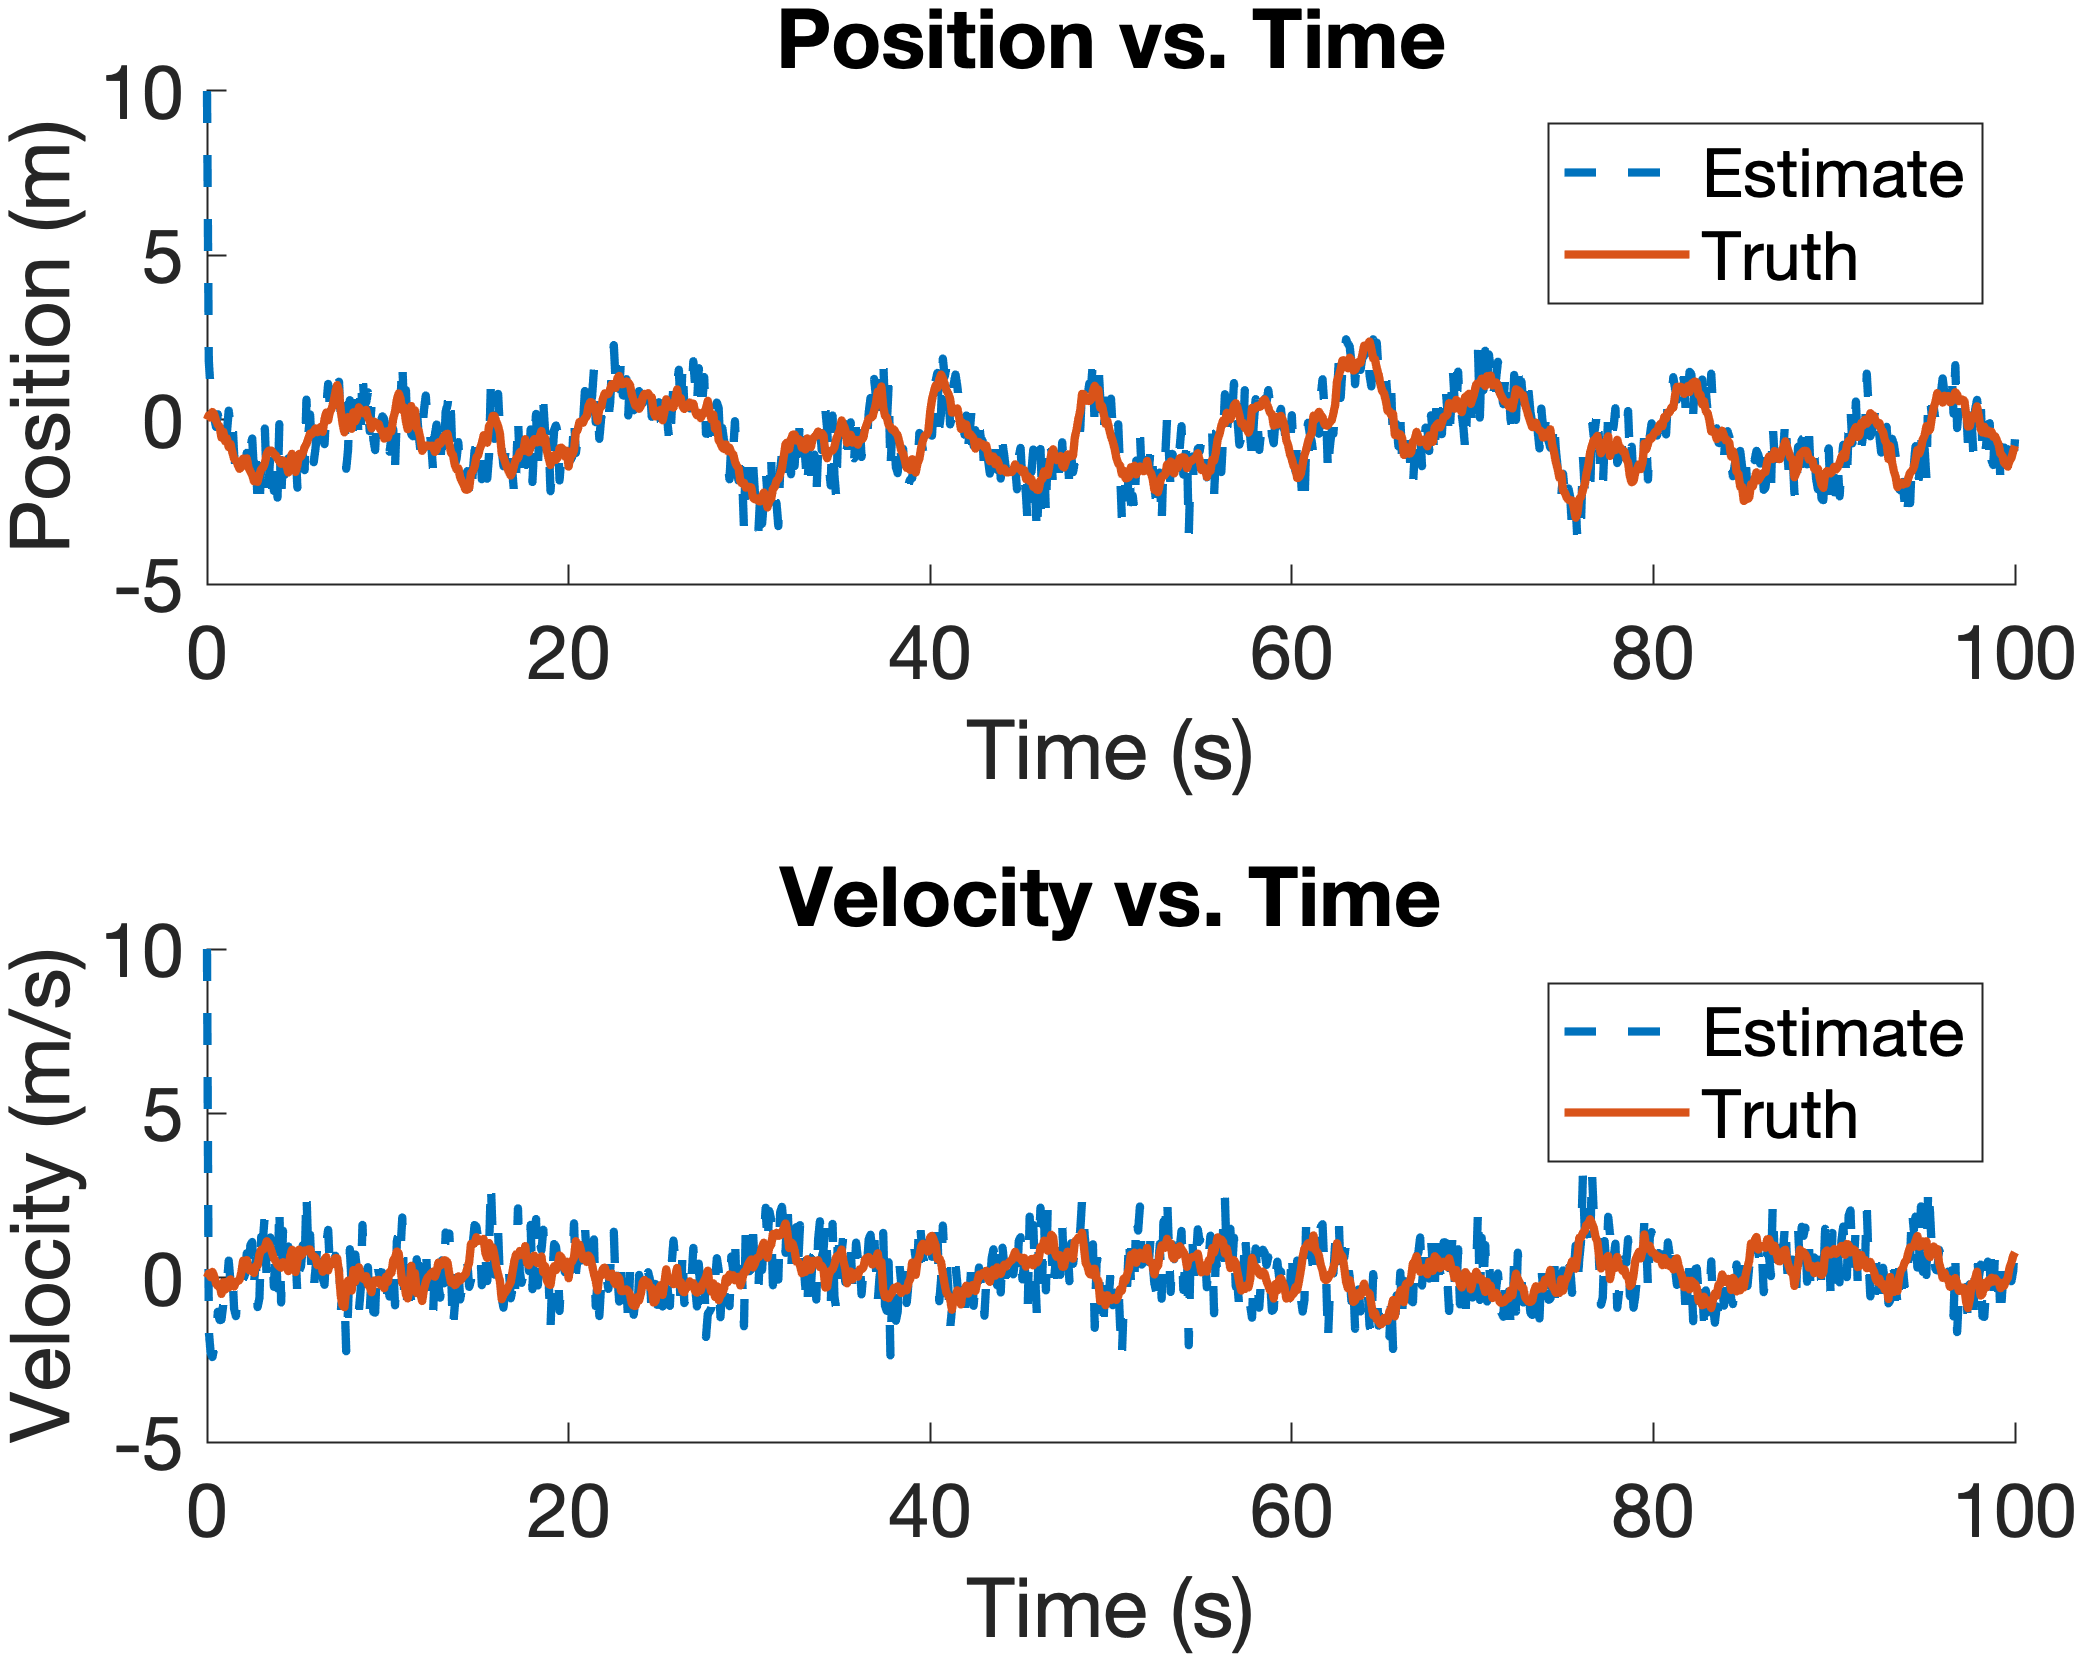
\includegraphics[width=0.75\linewidth]{../figures/p1d.png}
    \caption{SS Kalman Filter State Estimate vs. Time}\label{fig:p1d}
\end{figure}
\begin{gather*}
    N = 1.0816\\
    N_{ss} = 1.0788
\end{gather*}

\subsection*{Part E}
Change the ratio of the $Q$ and $R_d$ weights in the Kalman filter design (and repeat 
part d with the new Kalman gain but DO NOT regenerate a new $x$ and $\dot{x}$) and 
determine the effect on the estimation errors.  For what ratio of $Q$ and $R_d$ are 
the errors minimized?  Note: Often in practice we do not know the actual $Q$ and $R_d$
so these tend to be "tuning" parameters we use to tune our filter. However, according 
to Kalman, the estimation errors are only minimized if we use the $Q$ and $R_d$ of the 
physical system.
\subsection*{Solution}
It appears the norm of the estimate errors are minimized when $Q_c=4$ and $R_d=1$ which makes sense as that is the systems true noise values and 
Kalman stated it was at the system true values that the filter was optimal.

\section*{Question II}
Download the data hw3\textunderscore2 from the website.  The data is in the form 
$\begin{bmatrix} t & y \end{bmatrix}$.  Suppose we want to design an estimator to 
estimate the bias in the measurement $y$.  We believe the bias $(x)$ is constant so we 
use the model given by:
\begin{gather}
    \dot{x} = 0\\
    y_k = x_k + \nu_k\\
    \nu_k\sim N(0,1)
\end{gather}
\subsection*{Part A}
Run the Kalman filter estimator with $Q_d=0$.  What happnes at $t>100$ seconds? Why? Calculate the steady state Kalman gain $L_{ss}$. Plot $L(k)$.  
This is known as the filter "going to sleep" (becomes a least squares estimator).
\subsection*{Solution}
\begin{figure}[H]
    \centering
    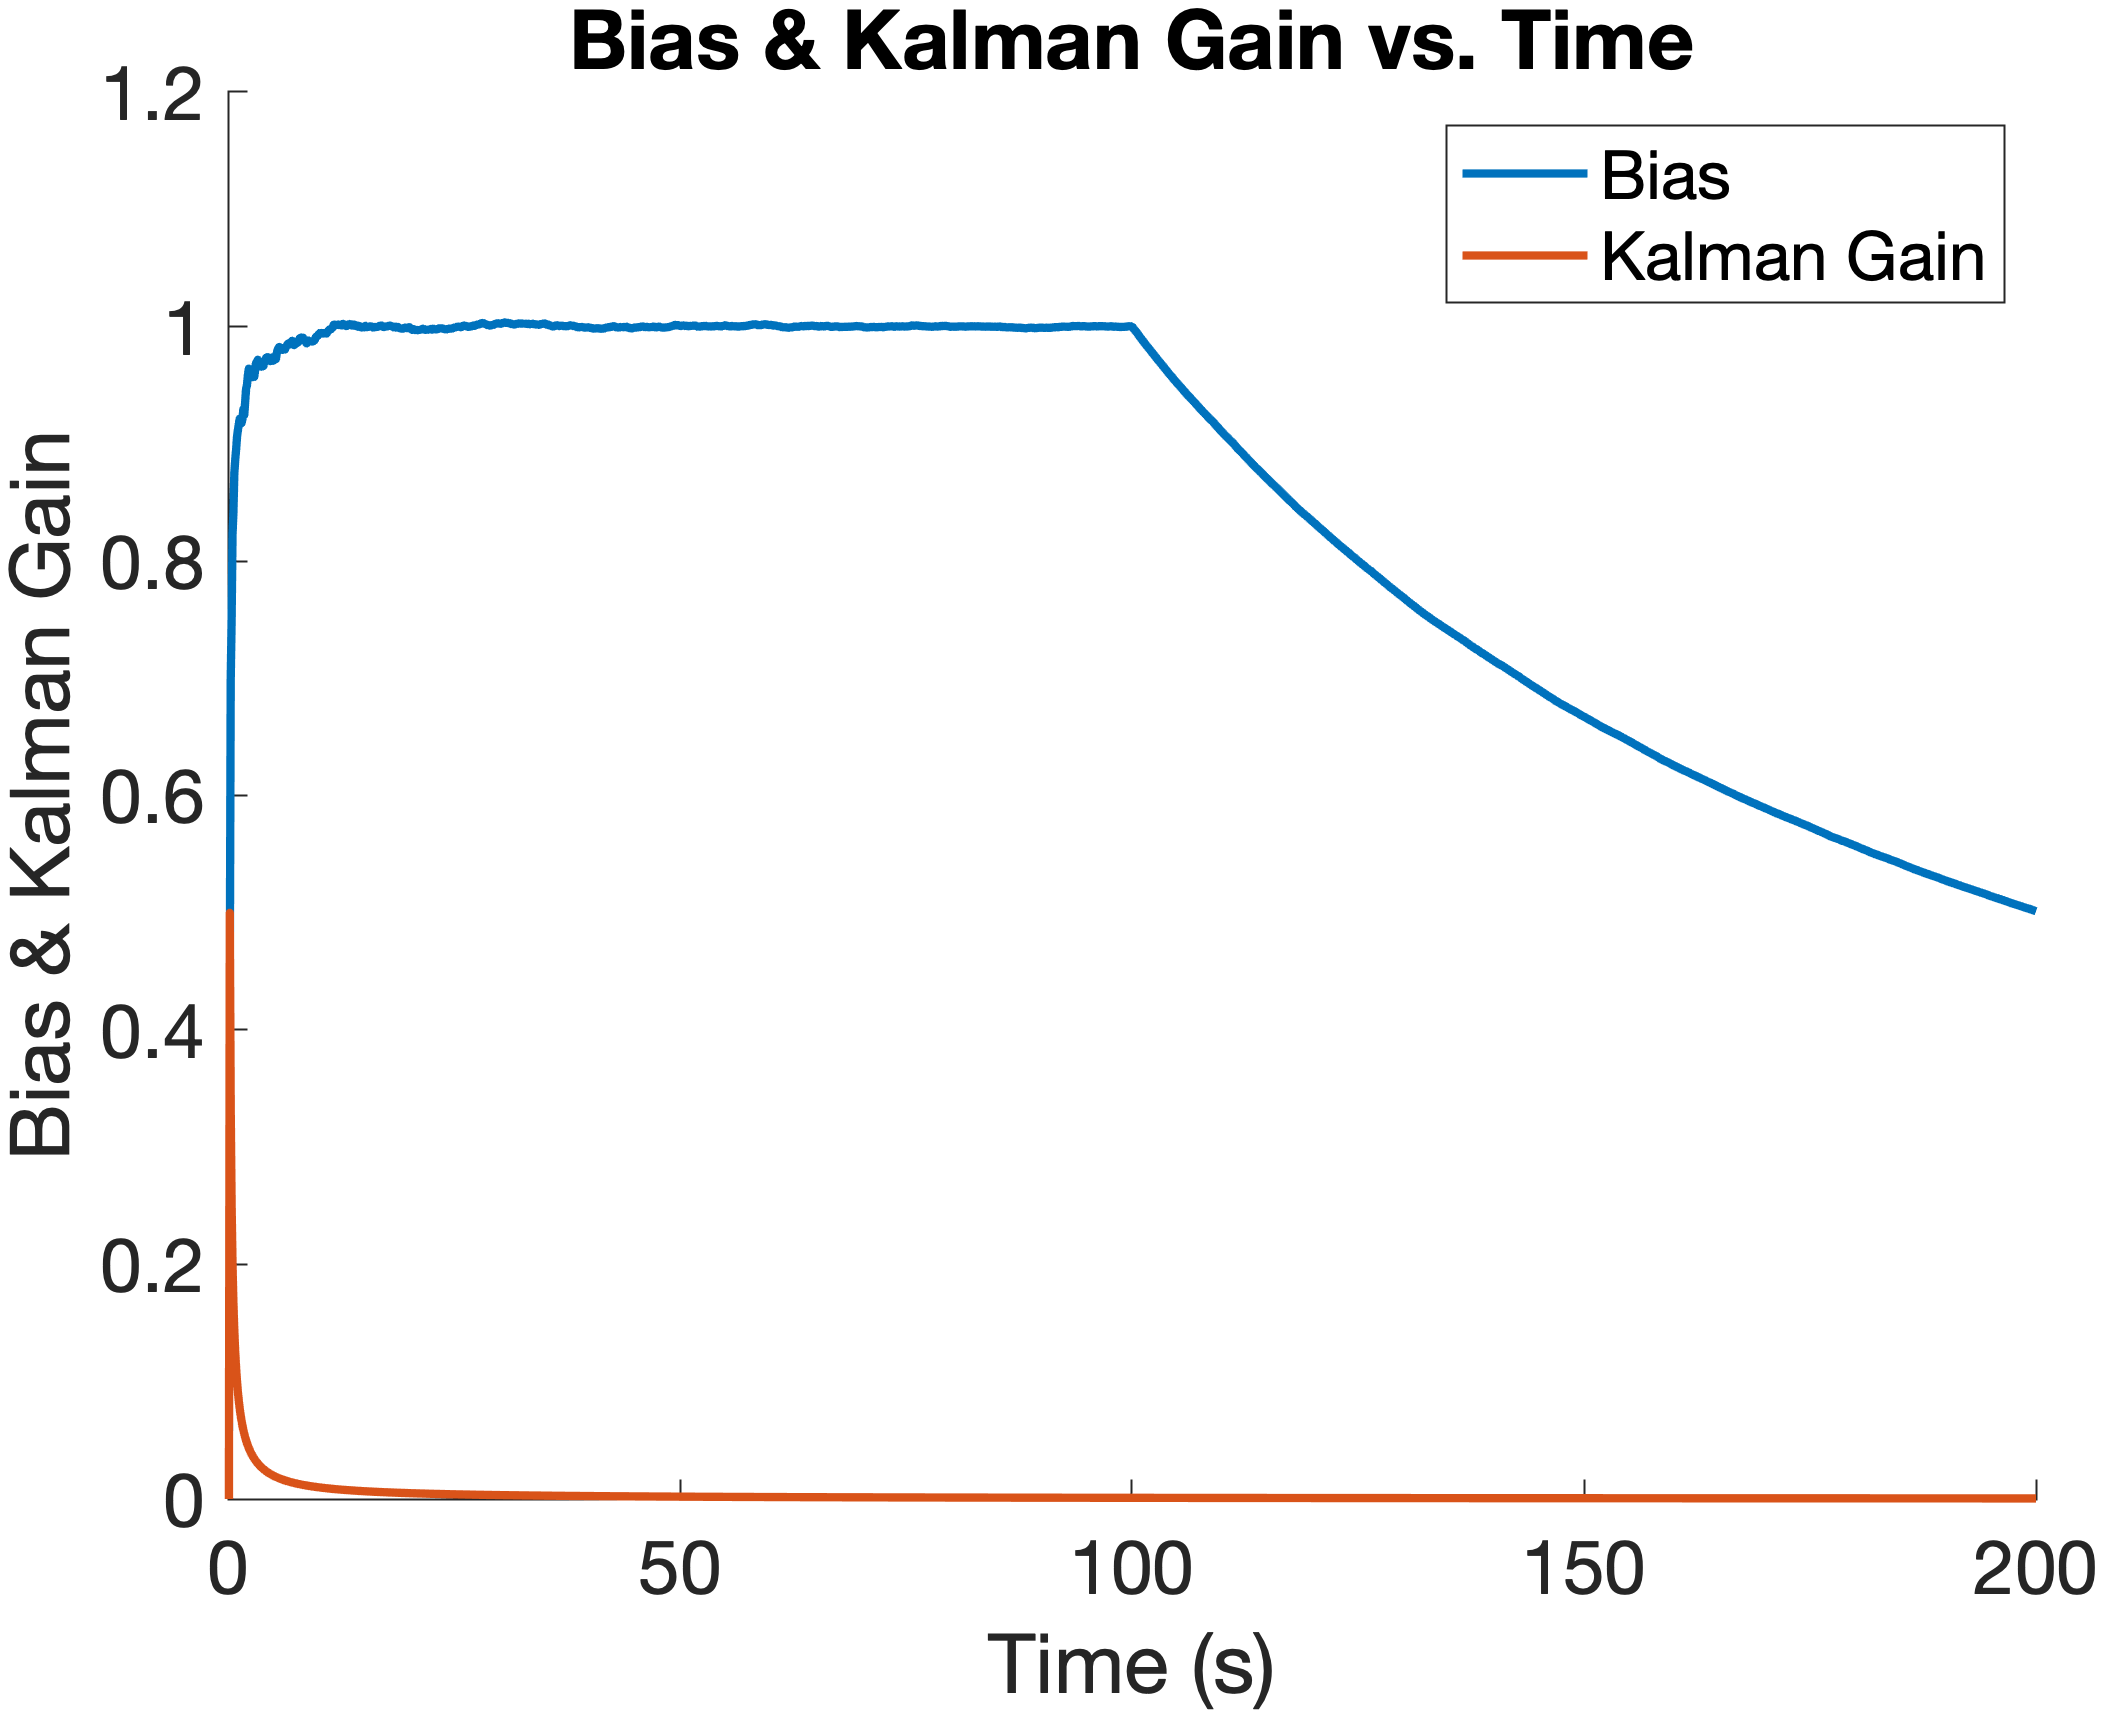
\includegraphics[width=0.75\linewidth]{../figures/p2a.png}
    \caption{Bias \& Kalman Gain vs. Time}\label{fig:p2a}
\end{figure}
At $t>100$, the estimate of the bias slowly starts to decrease.  The actual bias has a step change in it's value and the Kalman Filter is trying 
to estimate that.  The Kalman Filter has "gone to sleep" though, and is no longer accurately estimating the state.   This can be inferred from the 
steady-state value of the Kalman gain:
\begin{gather*}
    L_{ss} = 0
\end{gather*}

\subsection*{Part B}
To offset this problem we will "tune" $Q_d$ to track the bias.  What is the effect of changing $Q_d$ on the ability to track the step change in the 
bias? (try values of $Q_d$ from 0.0001 to 0.01 and plot $L(k)$ as well as the estimate of the bias $(\hat{x})$).  What is the tradeoff?
\subsection*{Solution}
\begin{figure}[H]
    \centering
    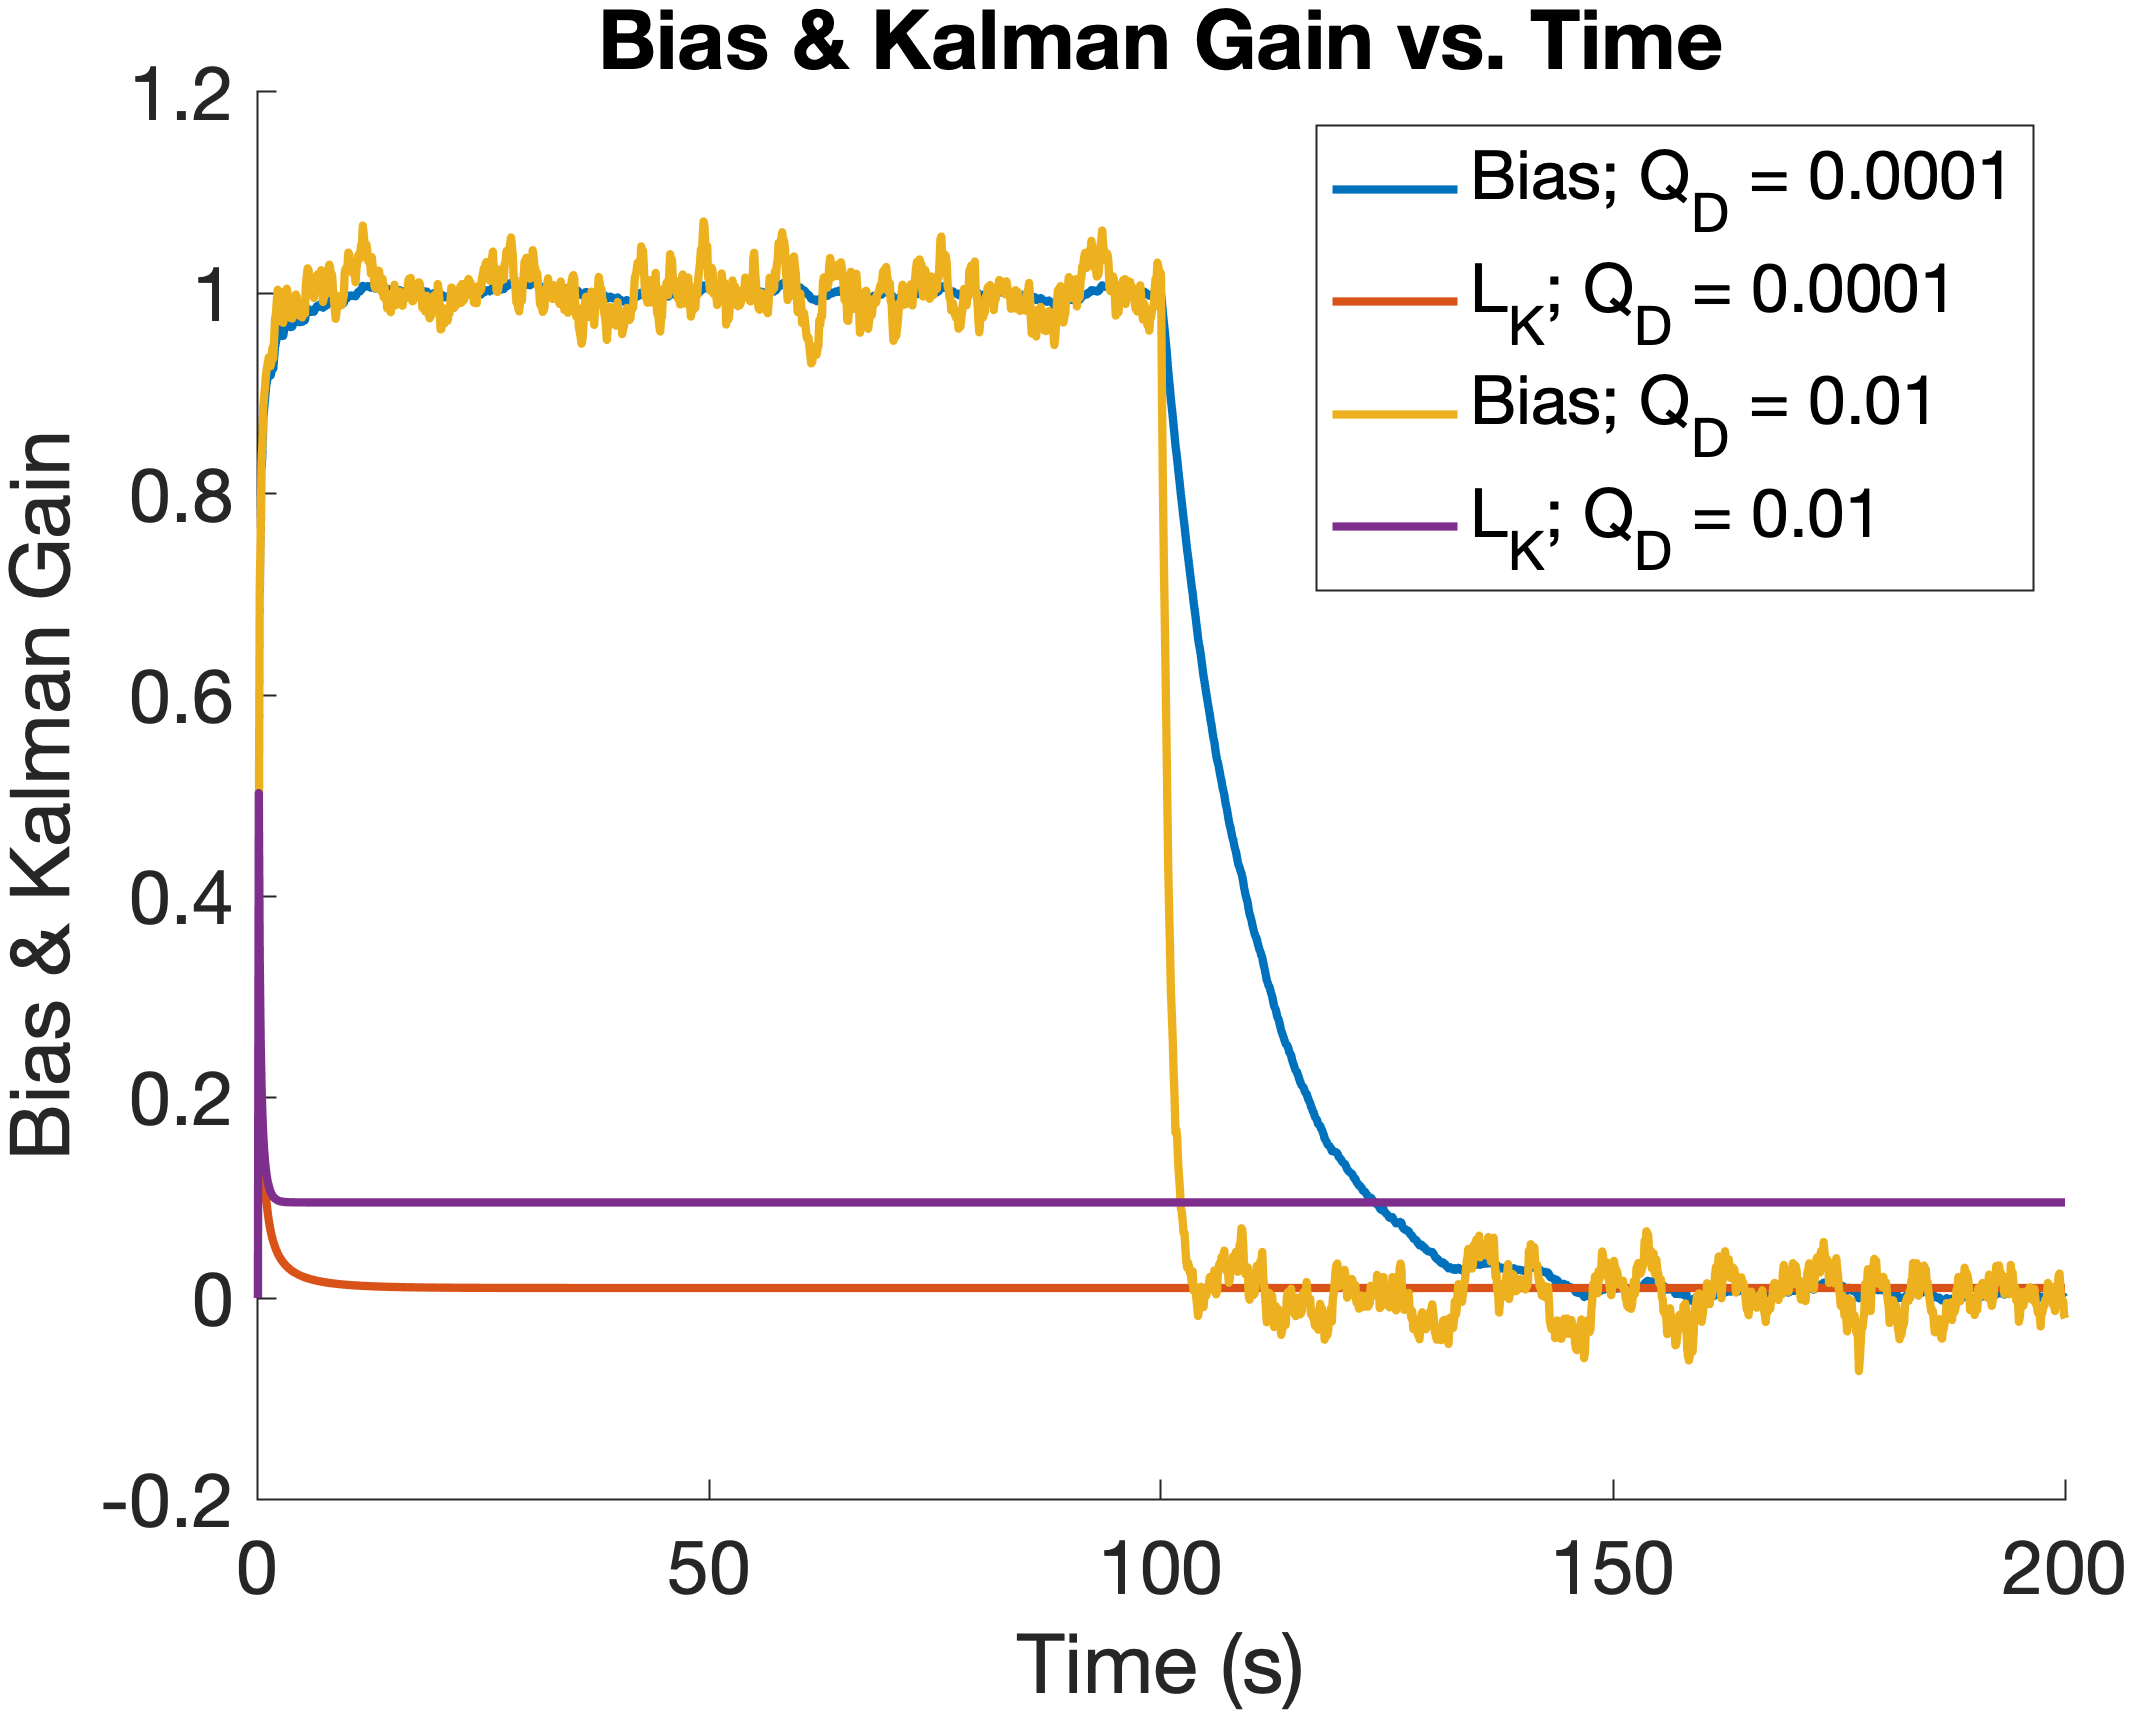
\includegraphics[width=0.75\linewidth]{../figures/p2b.png}
    \caption{Bias \& Kalman Gain vs. Time}\label{fig:p2b}
\end{figure}
The tradeoff with higher $Q_d$ values is better/"faster" tracking of the estimate, though by gaining more noise on the estimate.

\subsection*{Part C}
Now filter the measurement using the first order low-pass filter:
\begin{gather}
    H(z)=\frac{sqrt{Q_d}}{z - (1-sqrt{Q_d})}
\end{gather}
us ethe command: yf = filter(numd, dend, y, y0)
\subsection*{Solution}
\begin{figure}[H]
    \centering
    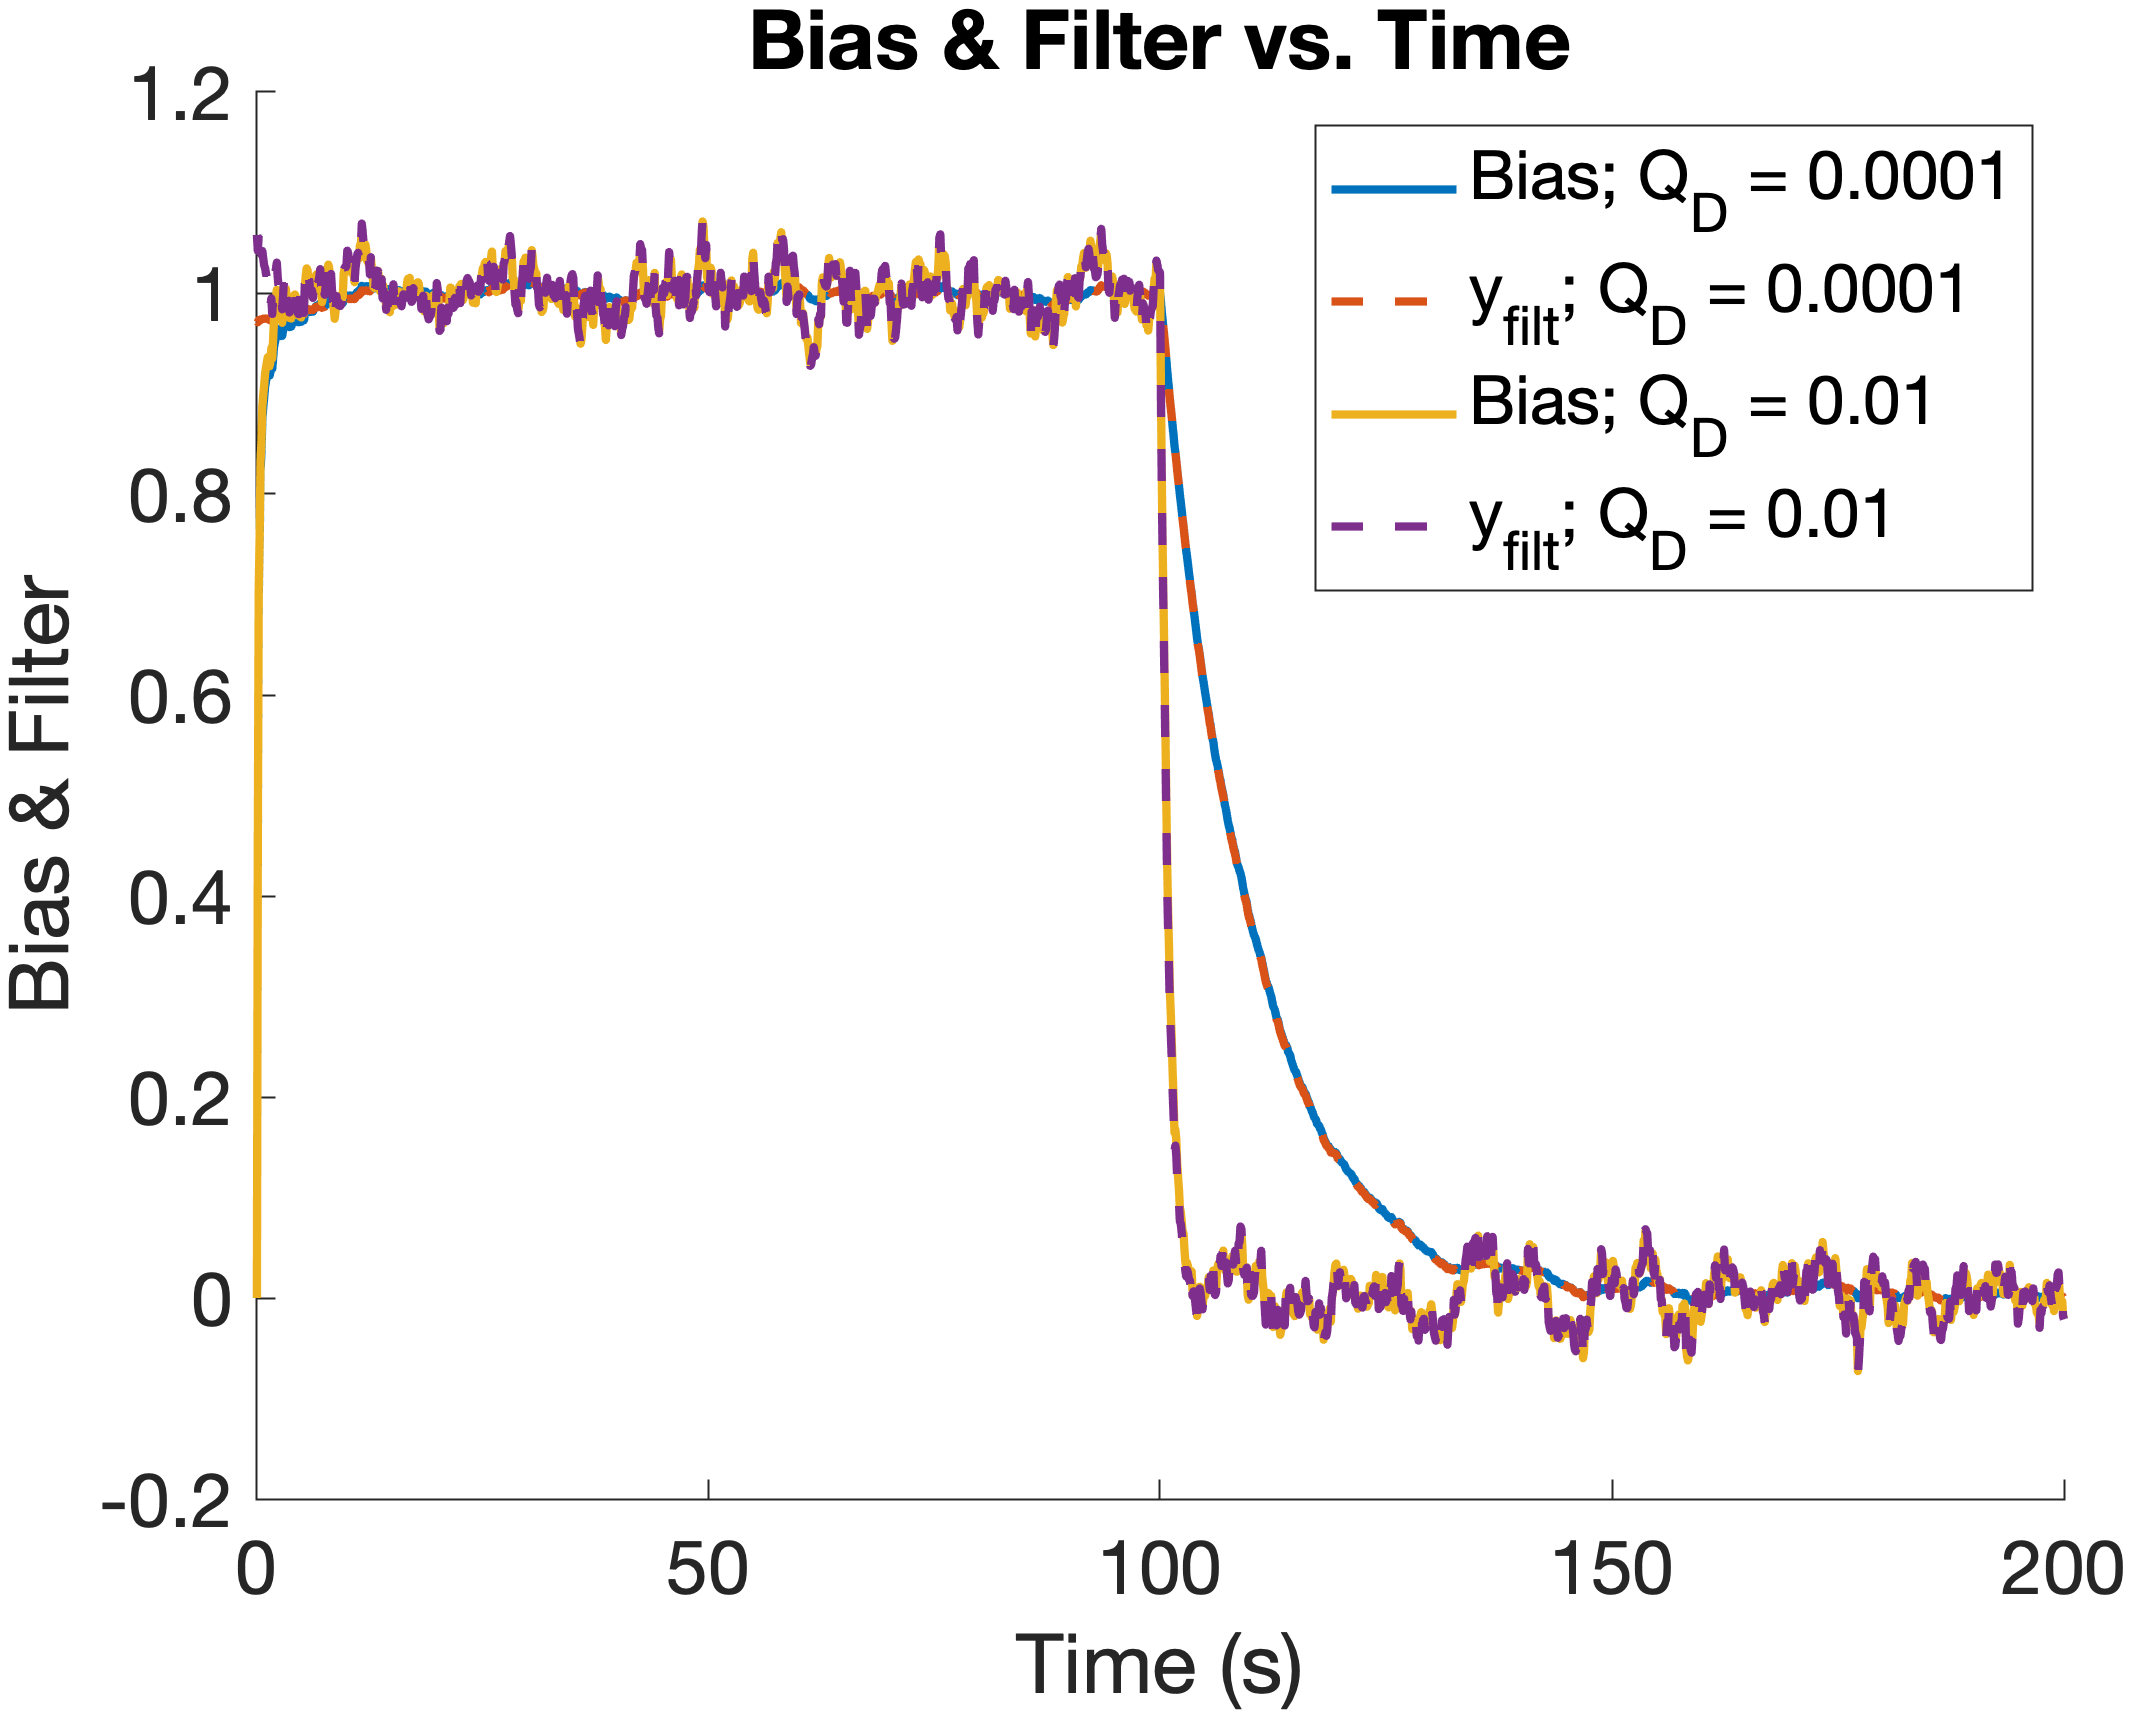
\includegraphics[width=0.75\linewidth]{../figures/p2c.png}
    \caption{Bias \& Filter vs. Time}\label{fig:p2c}
\end{figure}

\subsection*{Part D}
How does this compare to the Kalman filter solution.  Why are these two filters the same for this problem?
\subsection*{Solution}
The filtered signal and the Kalman Filter estimate match exactly.  The Kalman Filter for this setup has no time update.  It is just using measurements $(y)$ to filter the process noise $Q_d$ which leaves the bias.  This is exactly what the provided filter is doing as well.

\section*{Question III}
Design a “Navigation” type Kalman filter to estimate the states [East, North,
Radar\textunderscore Bias, Psi, Gyro\textunderscore Bias]. (Note: this is a non-linear problem that requires an
Extended Kalman Filter (EKF) to do correctly). However we can solve the problem in
one of two ways: (i) linearize the equations about the nominal operating point and
produce a constant A matrix for that operating point, or (ii) simply update the A matrix
at every time step with our measurements or estimates. Download the data hw3\textunderscore3
from the website and run the filter sampled at 5 Hz
\subsection*{Part A}
How did you choose the covariance values for $Q_d$ (especially for the radar and gyro biases).
\subsection*{Solution}
Before beginning to form the state-space model of the filter the states being estimated needed to be identified.
\begin{gather*}
    x = \begin{bmatrix}
        E \\ N \\ \psi \\ b_r \\ b_g
    \end{bmatrix}
\end{gather*}
With the states identified, equations relating the measurements to those states need to be identified.
\begin{gather*}
    y = \begin{bmatrix}
        \tilde{E} \\ \tilde{N} \\ \tilde{\psi} \\ \dot{\tilde{\psi}} \\ \tilde{V}
    \end{bmatrix} \\
    \tilde{E} = E + \nu_E\\
    \tilde{N} = N + \nu_N\\
    \tilde{\psi} = \psi + \nu_\psi\\
    \dot{\tilde{\psi}} = \dot{\psi} + b_g + \omega_g\\
    \tilde{V} = V + b_r + \omega_r
\end{gather*}
With the states and measurement equations identified, the last step before forming the state-space representation is to identify equations for the state derivatives.
\begin{gather*}
    \dot{E} = V\sin(\psi) = (\tilde{V} - b_r - \omega_r)\sin(\psi)\\
    \dot{N} = V\cos(\psi) = (\tilde{V} - b_r - \omega_r)\cos(\psi)\\
    \dot{\psi} = \dot{\psi} = \dot{\tilde{\psi}} - b_g - \omega_g\\
    \dot{b_r} = 0\\
    \dot{b_g} = 0
\end{gather*}
With all the equations identified, the state space representation can start to take form.  This begins with identifying $f(x)$ and $h(x)$ and taking their Jacobians.
\begin{gather*}
    \dot{x} = f(x) = \begin{bmatrix}
        (\tilde{V} - b_r)\sin(\psi)\\
        (\tilde{V} - b_r)\cos(\psi)\\
        \dot{\tilde{\psi}} - b_g\\
        0\\
        0
    \end{bmatrix} y = h(x) = \begin{bmatrix}
        E\\
        N\\
        \psi\\
        \dot{\psi} + b_g\\
        V + b_r
    \end{bmatrix}\\
    A = \frac{\partial f}{\partial x} = \begin{bmatrix}
        0 & 0 & (\tilde{V}-b_r)\cos(\psi) & -\sin(\psi) & 0\\
        0 & 0 & (\tilde{V}-b_r)\cos(\psi) & -\cos(\psi) & 0\\
        0 & 0 & 0 & 0 & -1\\
        0 & 0 & 0 & 0 & 0\\
        0 & 0 & 0 & 0 & 0\\
    \end{bmatrix}\\
    H = \frac{\partial h}{\partial x} = \begin{bmatrix}
        1 & 0 & 0 & 0 & 0\\
        0 & 1 & 0 & 0 & 0\\
        0 & 0 & 1 & 0 & 0\\
        0 & 0 & 0 & 0 & 1\\
        0 & 0 & 0 & 1 & 0\\
    \end{bmatrix}
\end{gather*}
Now with all equations and Jacobians identified and solved, the normal Kalman Filter techniques can be applied.  The results are presented below.
\begin{figure}[H]
    \centering
    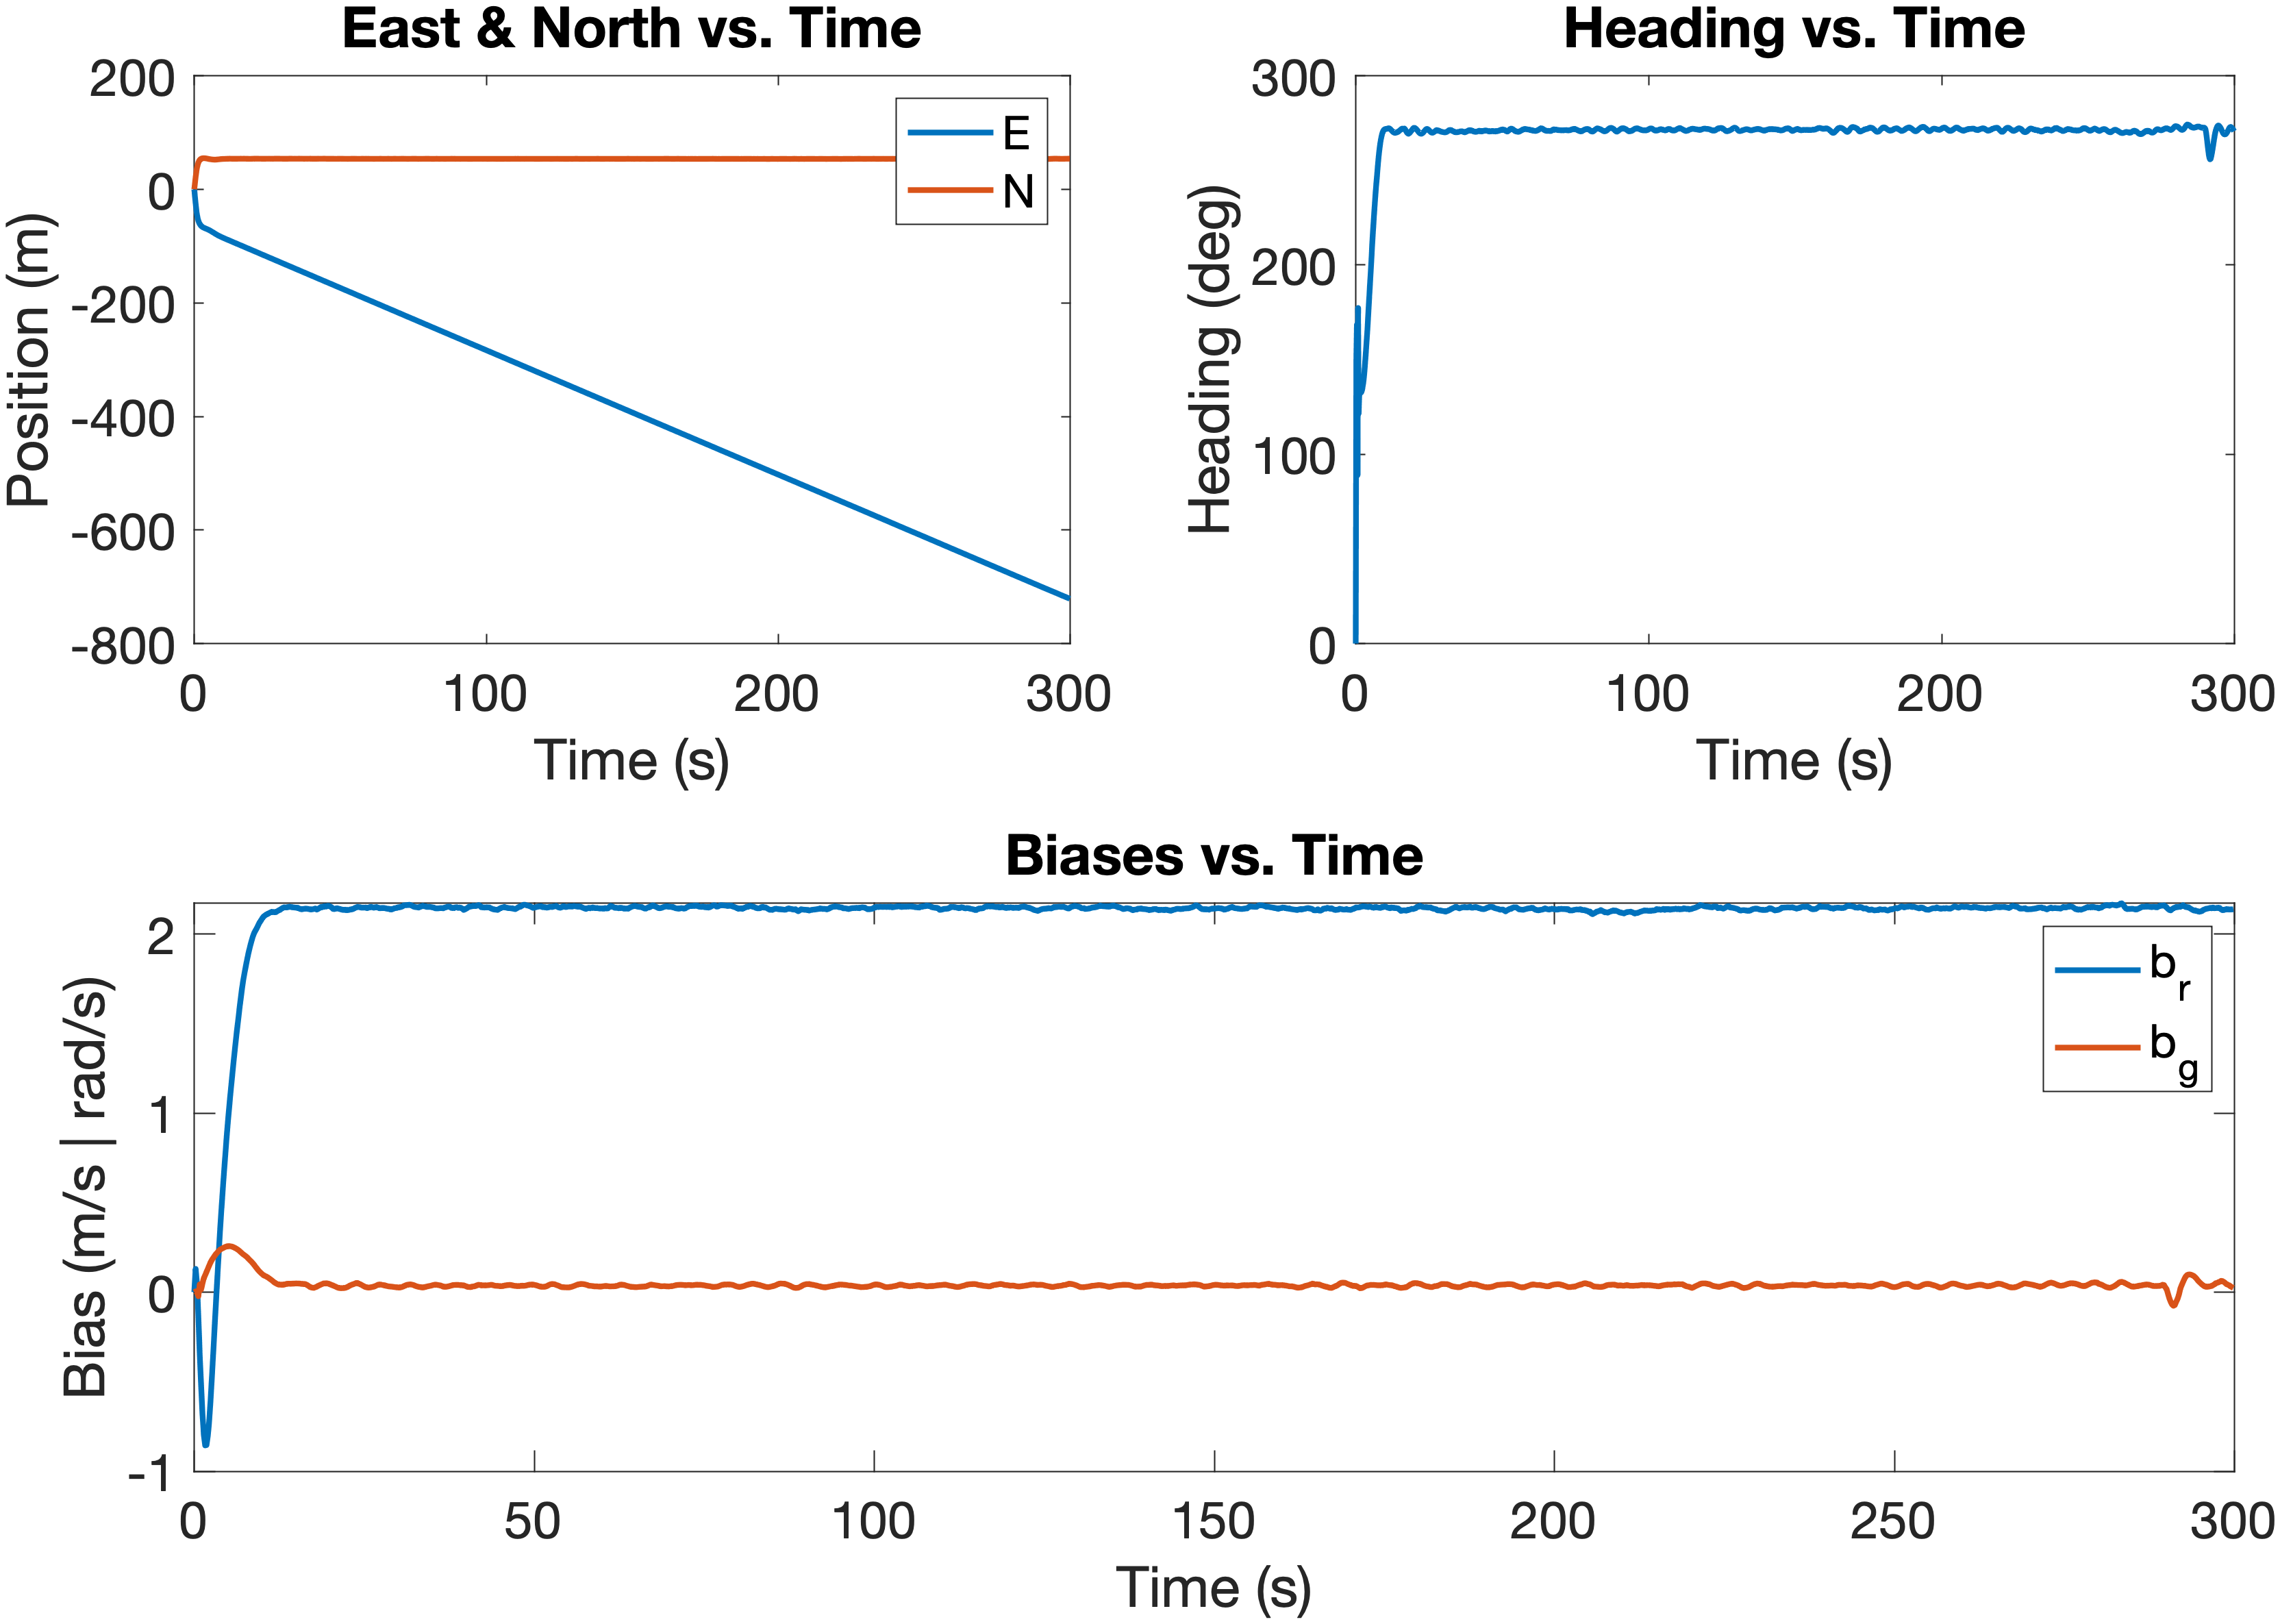
\includegraphics[width=0.75\linewidth]{../figures/p3a.png}
    \caption{Nav KF States vs. Time}\label{fig:p3a}
\end{figure}
$Q_d$ and $R_d$ were both tuned (starting at values of 1) until the estimate was consistent and noise was minimized on the estimates.  The matrices are as follows:
\begin{gather*}
    Q_d = \begin{bmatrix}
        0.01 & 0 & 0 & 0 & 0\\
        0 & 0.01 & 0 & 0 & 0\\
        0 & 0 & 0.01 & 0 & 0\\
        0 & 0 & 0 & 0.001 & 0\\
        0 & 0 & 0 & 0 & 0.001\\
    \end{bmatrix}\\
    R_d = \begin{bmatrix}
        0.1 & 0 & 0 & 0 & 0\\
        0 & 0.1 & 0 & 0 & 0\\
        0 & 0 & 0.1 & 0 & 0\\
        0 & 0 & 0 & 0.1 & 0\\
        0 & 0 & 0 & 0 & 0.1\\
    \end{bmatrix}
\end{gather*}

\subsection*{Part B}
How does the bias estimation compare to the Least Squares Solution. How does the bias estimate compare to the Recursive Least Squares solution if 
you make the covariance $(Q_d)$ of the bias estimates equal to zero.
\subsection*{Solution}
The Recursive Least Squares solution used the same observation matrix presented in Part A.
\begin{figure}[H]
    \centering
    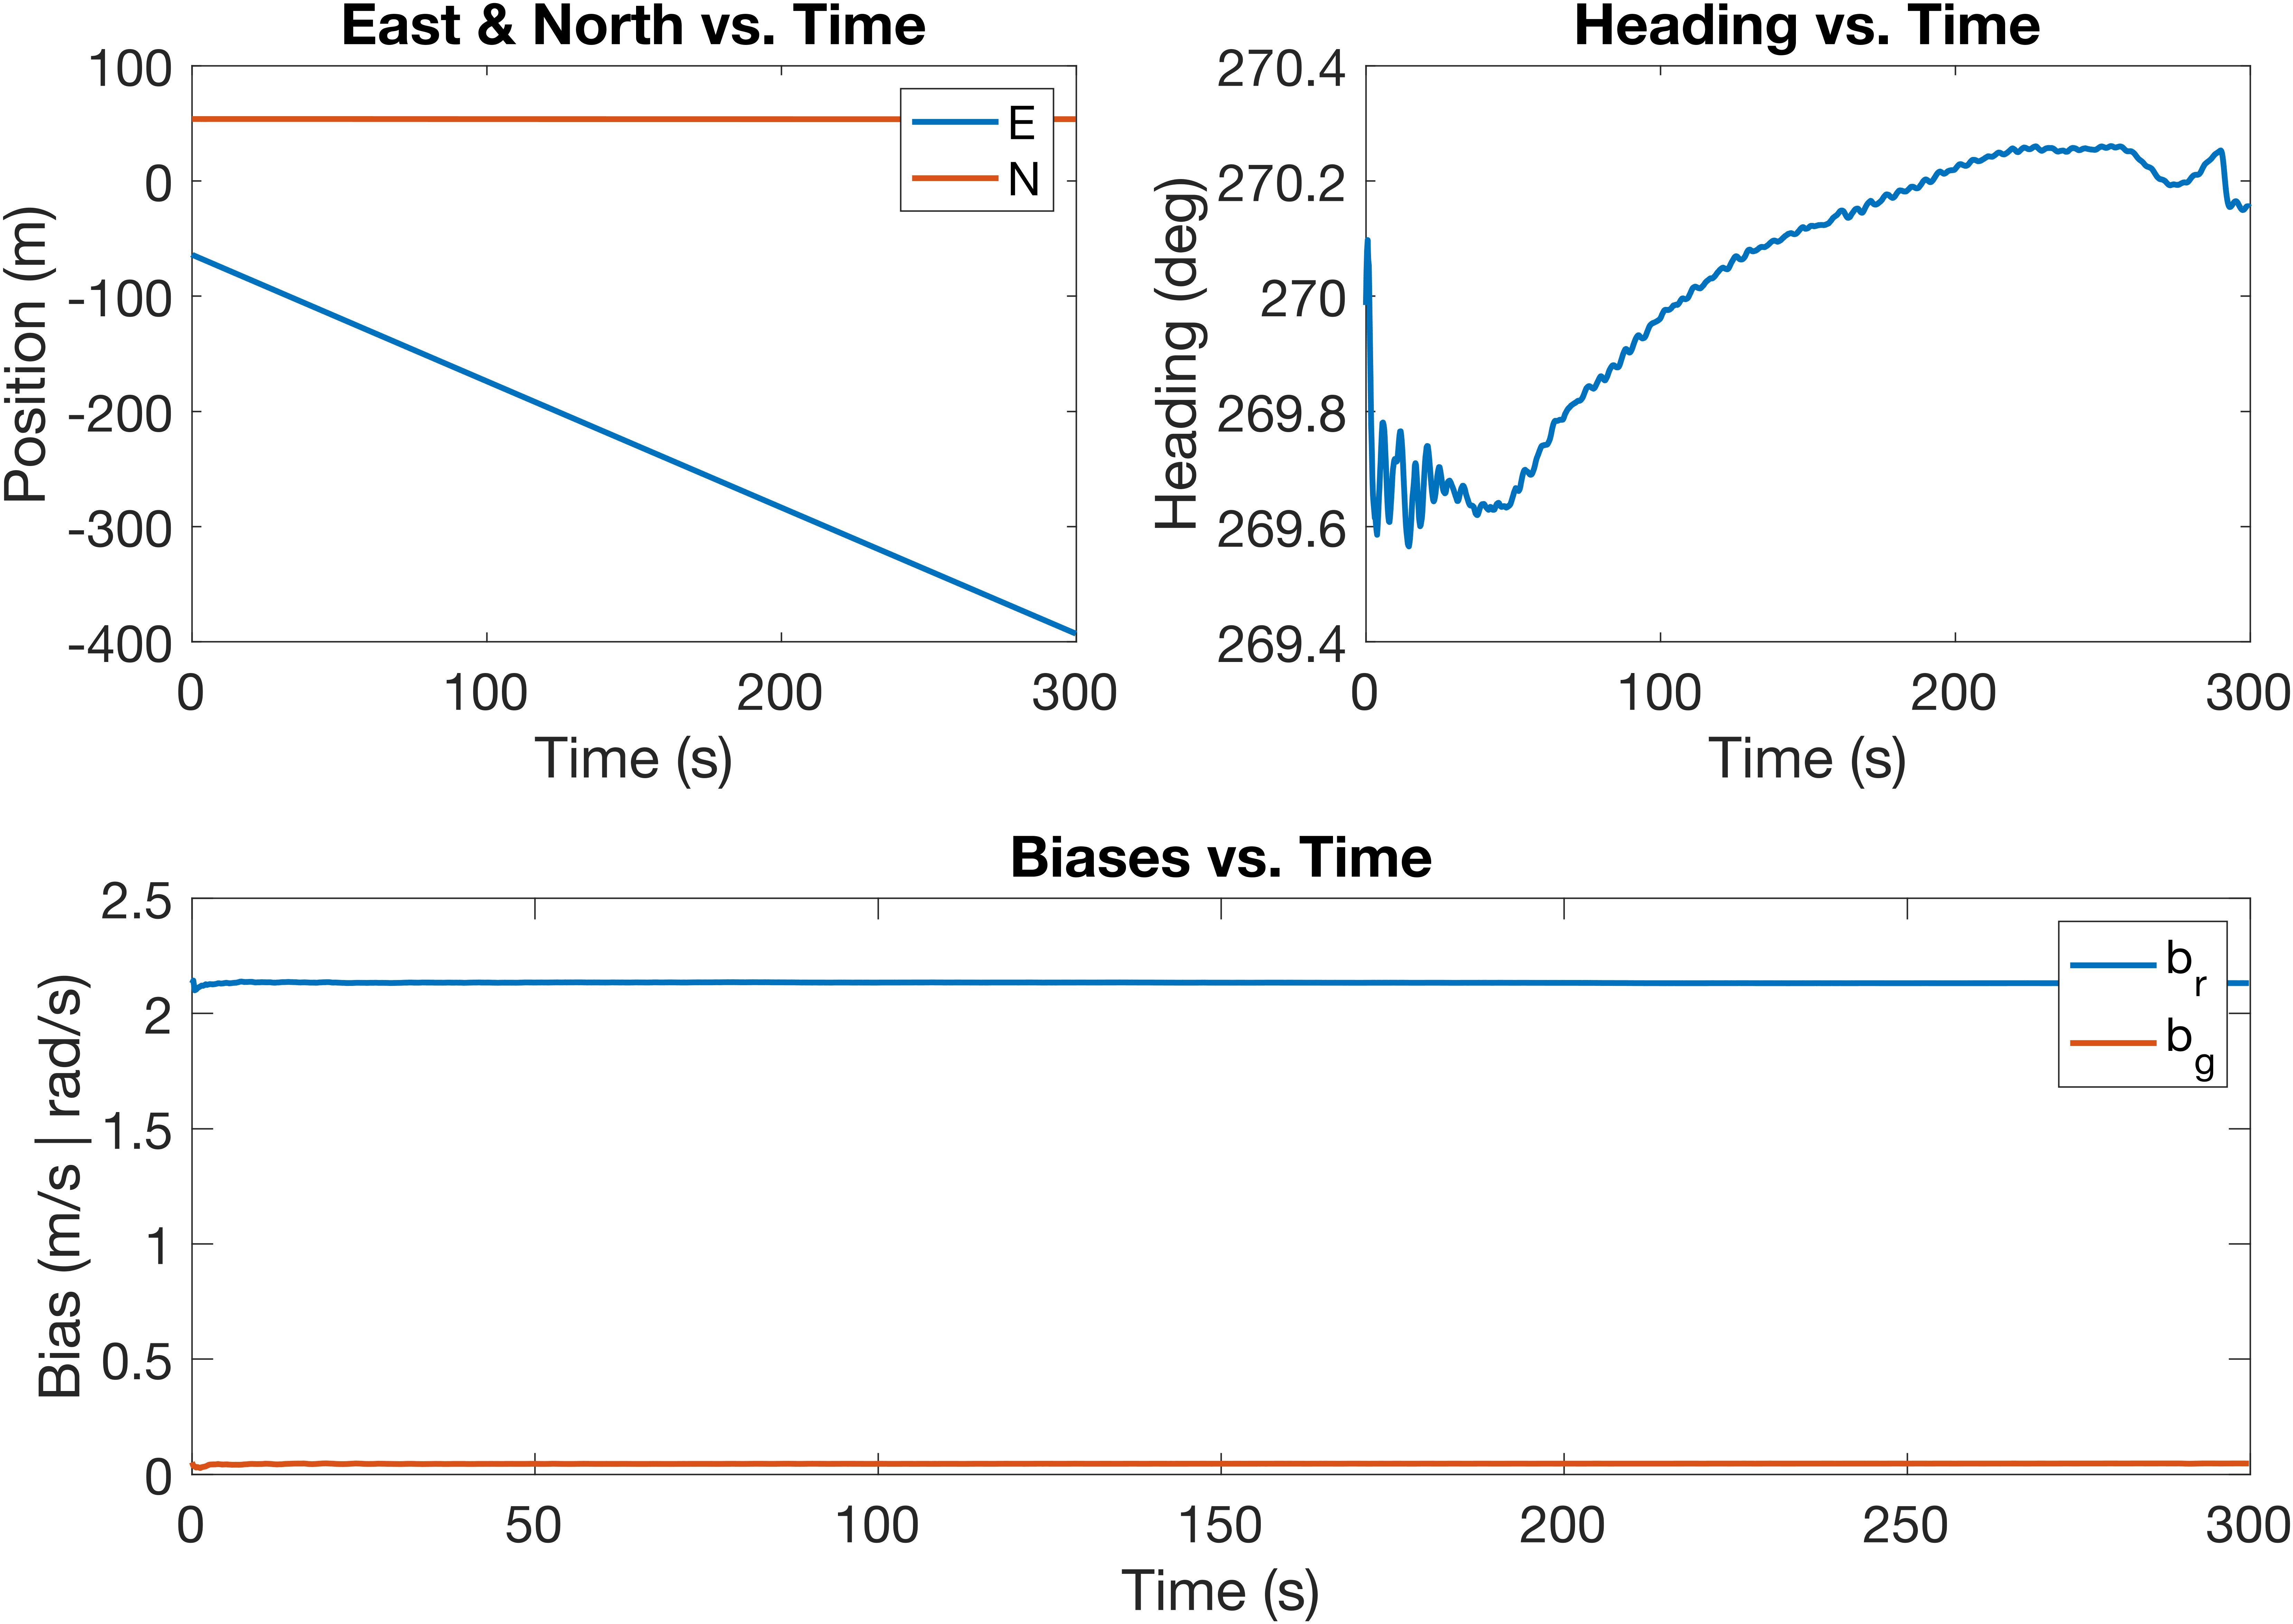
\includegraphics[width=0.75\linewidth]{../figures/p3b.png}
    \caption{Nav RLS States vs. Time}\label{fig:p3b}
\end{figure}
The bias estimates from the Recursive Least Squares (RLS) estimator match very closely with the Kalman Filter (KF) bias estimates.  It should be 
noted that the heading estimate is of a small scale, and the initial state "guess" isn't zero making it look noisier.  Looking at the plot scale 
shows this is a small magnitude of variation.

\subsection*{Part C}
Integrate the last 40 seconds of data to see how well you have estimated the biases.  This can simply be done by "turning off" the measurements 
in the observation matrix! Why do the bias estimates remain constant during the 40 second "outage?"
\subsection*{Solution}
\begin{figure}[H]
    \centering
    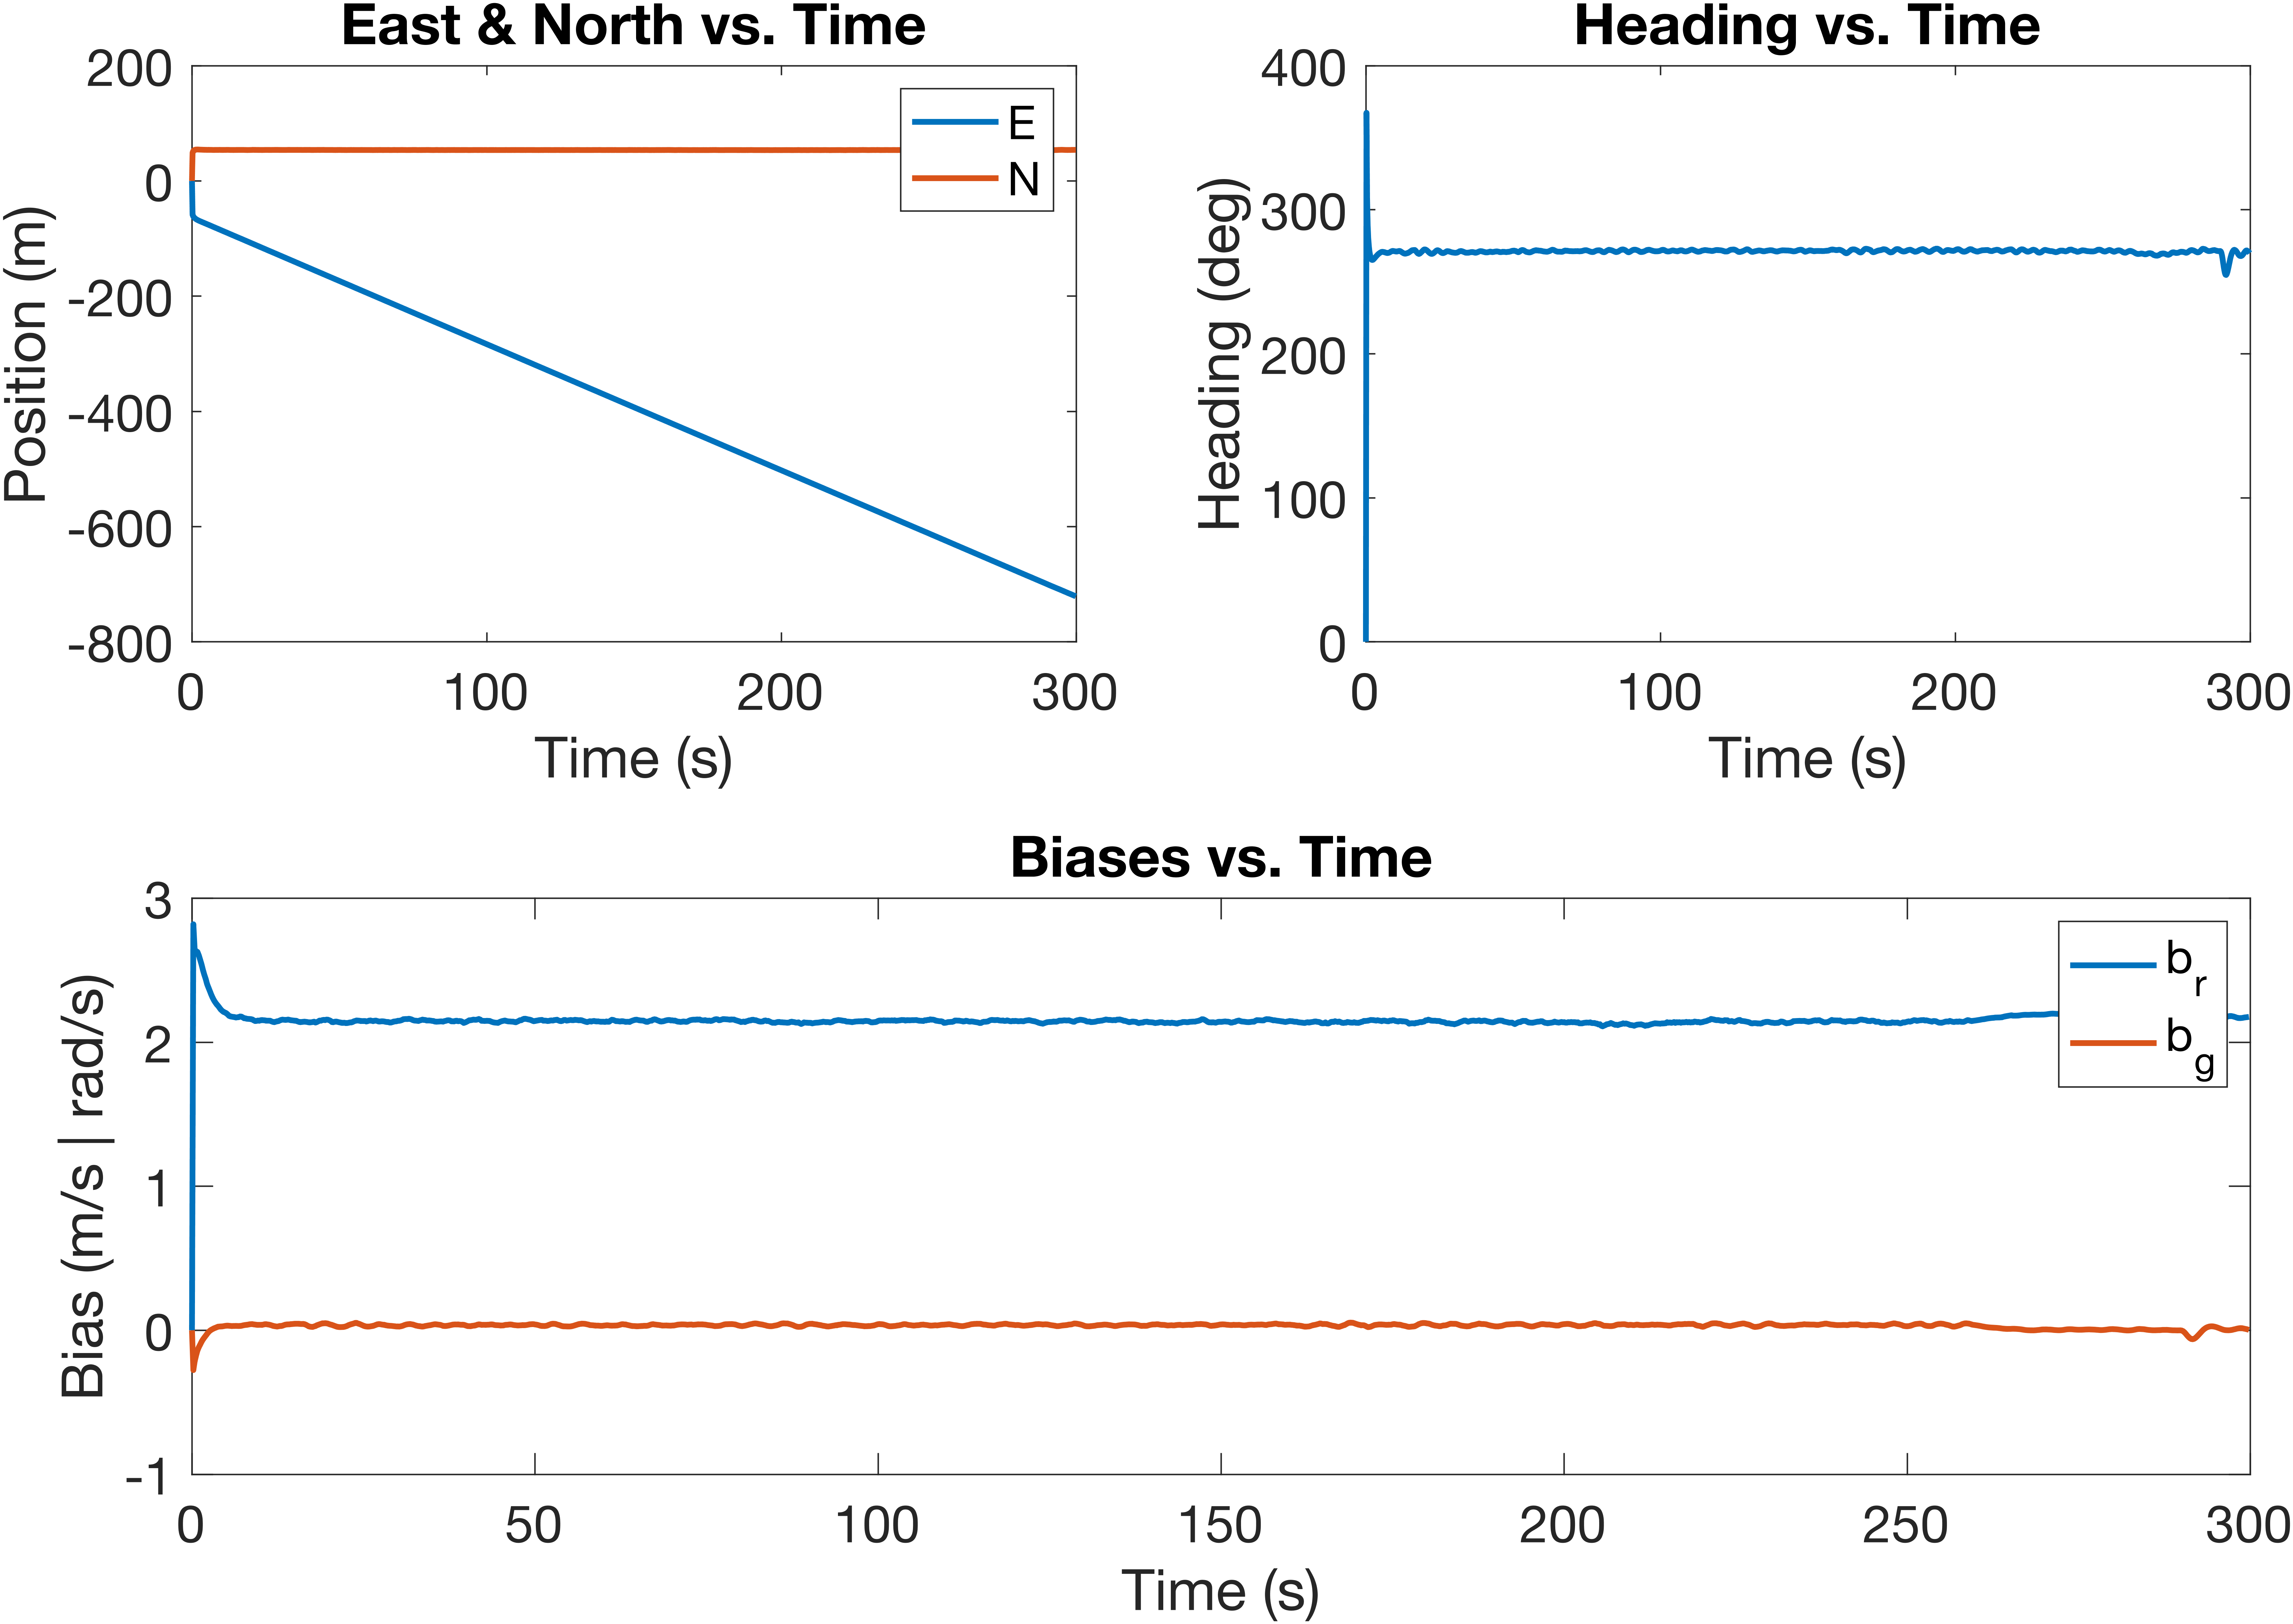
\includegraphics[width=0.75\linewidth]{../figures/p3c.png}
    \caption{Nav KF States w/ 40s "Outage" vs. Time}\label{fig:p3c}
\end{figure}
The biases remain fairly constant during the "outage" as they have no time update, and are now not being updated by the measurements either.

\section*{Question IV}
Estimate for Vehicle Dynamics. The yaw dynamics of a car (for a stability control system) can be described by the following model (at 25 m/s):
\begin{gather}
    \dot{X} = \begin{bmatrix}
        -2.62 & 12 \\
        -0.96 & -2
    \end{bmatrix}\begin{bmatrix}
        \dot{\Psi} \\
        \beta
    \end{bmatrix} + \begin{bmatrix}
        14 \\
        1
    \end{bmatrix}\delta \\
    y_k = \begin{bmatrix}
        1 & 0
    \end{bmatrix}X_k + \nu_k
\end{gather}
where:
\begin{gather}
    \dot{\Psi} - Vehicle Yaw Rate\\
    \beta - Vehicle Side Slip Angle\\
    \delta - Steer Angle\\
    \nu_k - Sample Sensor Noise
\end{gather}
\subsection*{Part A}
Assuming we can only measure the yaw rate $(\nu_k\sim N(0, 0.1^2))$, design a Kalman filter to do full state estimation (select a reasonable $Q_d$). Provide a unit step stee input and estimate both states.  On one page plot the actual states and estimated states (use subplot(2,2,n) for each of the two states). Where are the steady state poles of the estimator?
\subsection*{Solution}
Below is a plot of the simulated system yaw-rate vs. the simulated measurement thereof.
\begin{figure}[H]
    \centering
    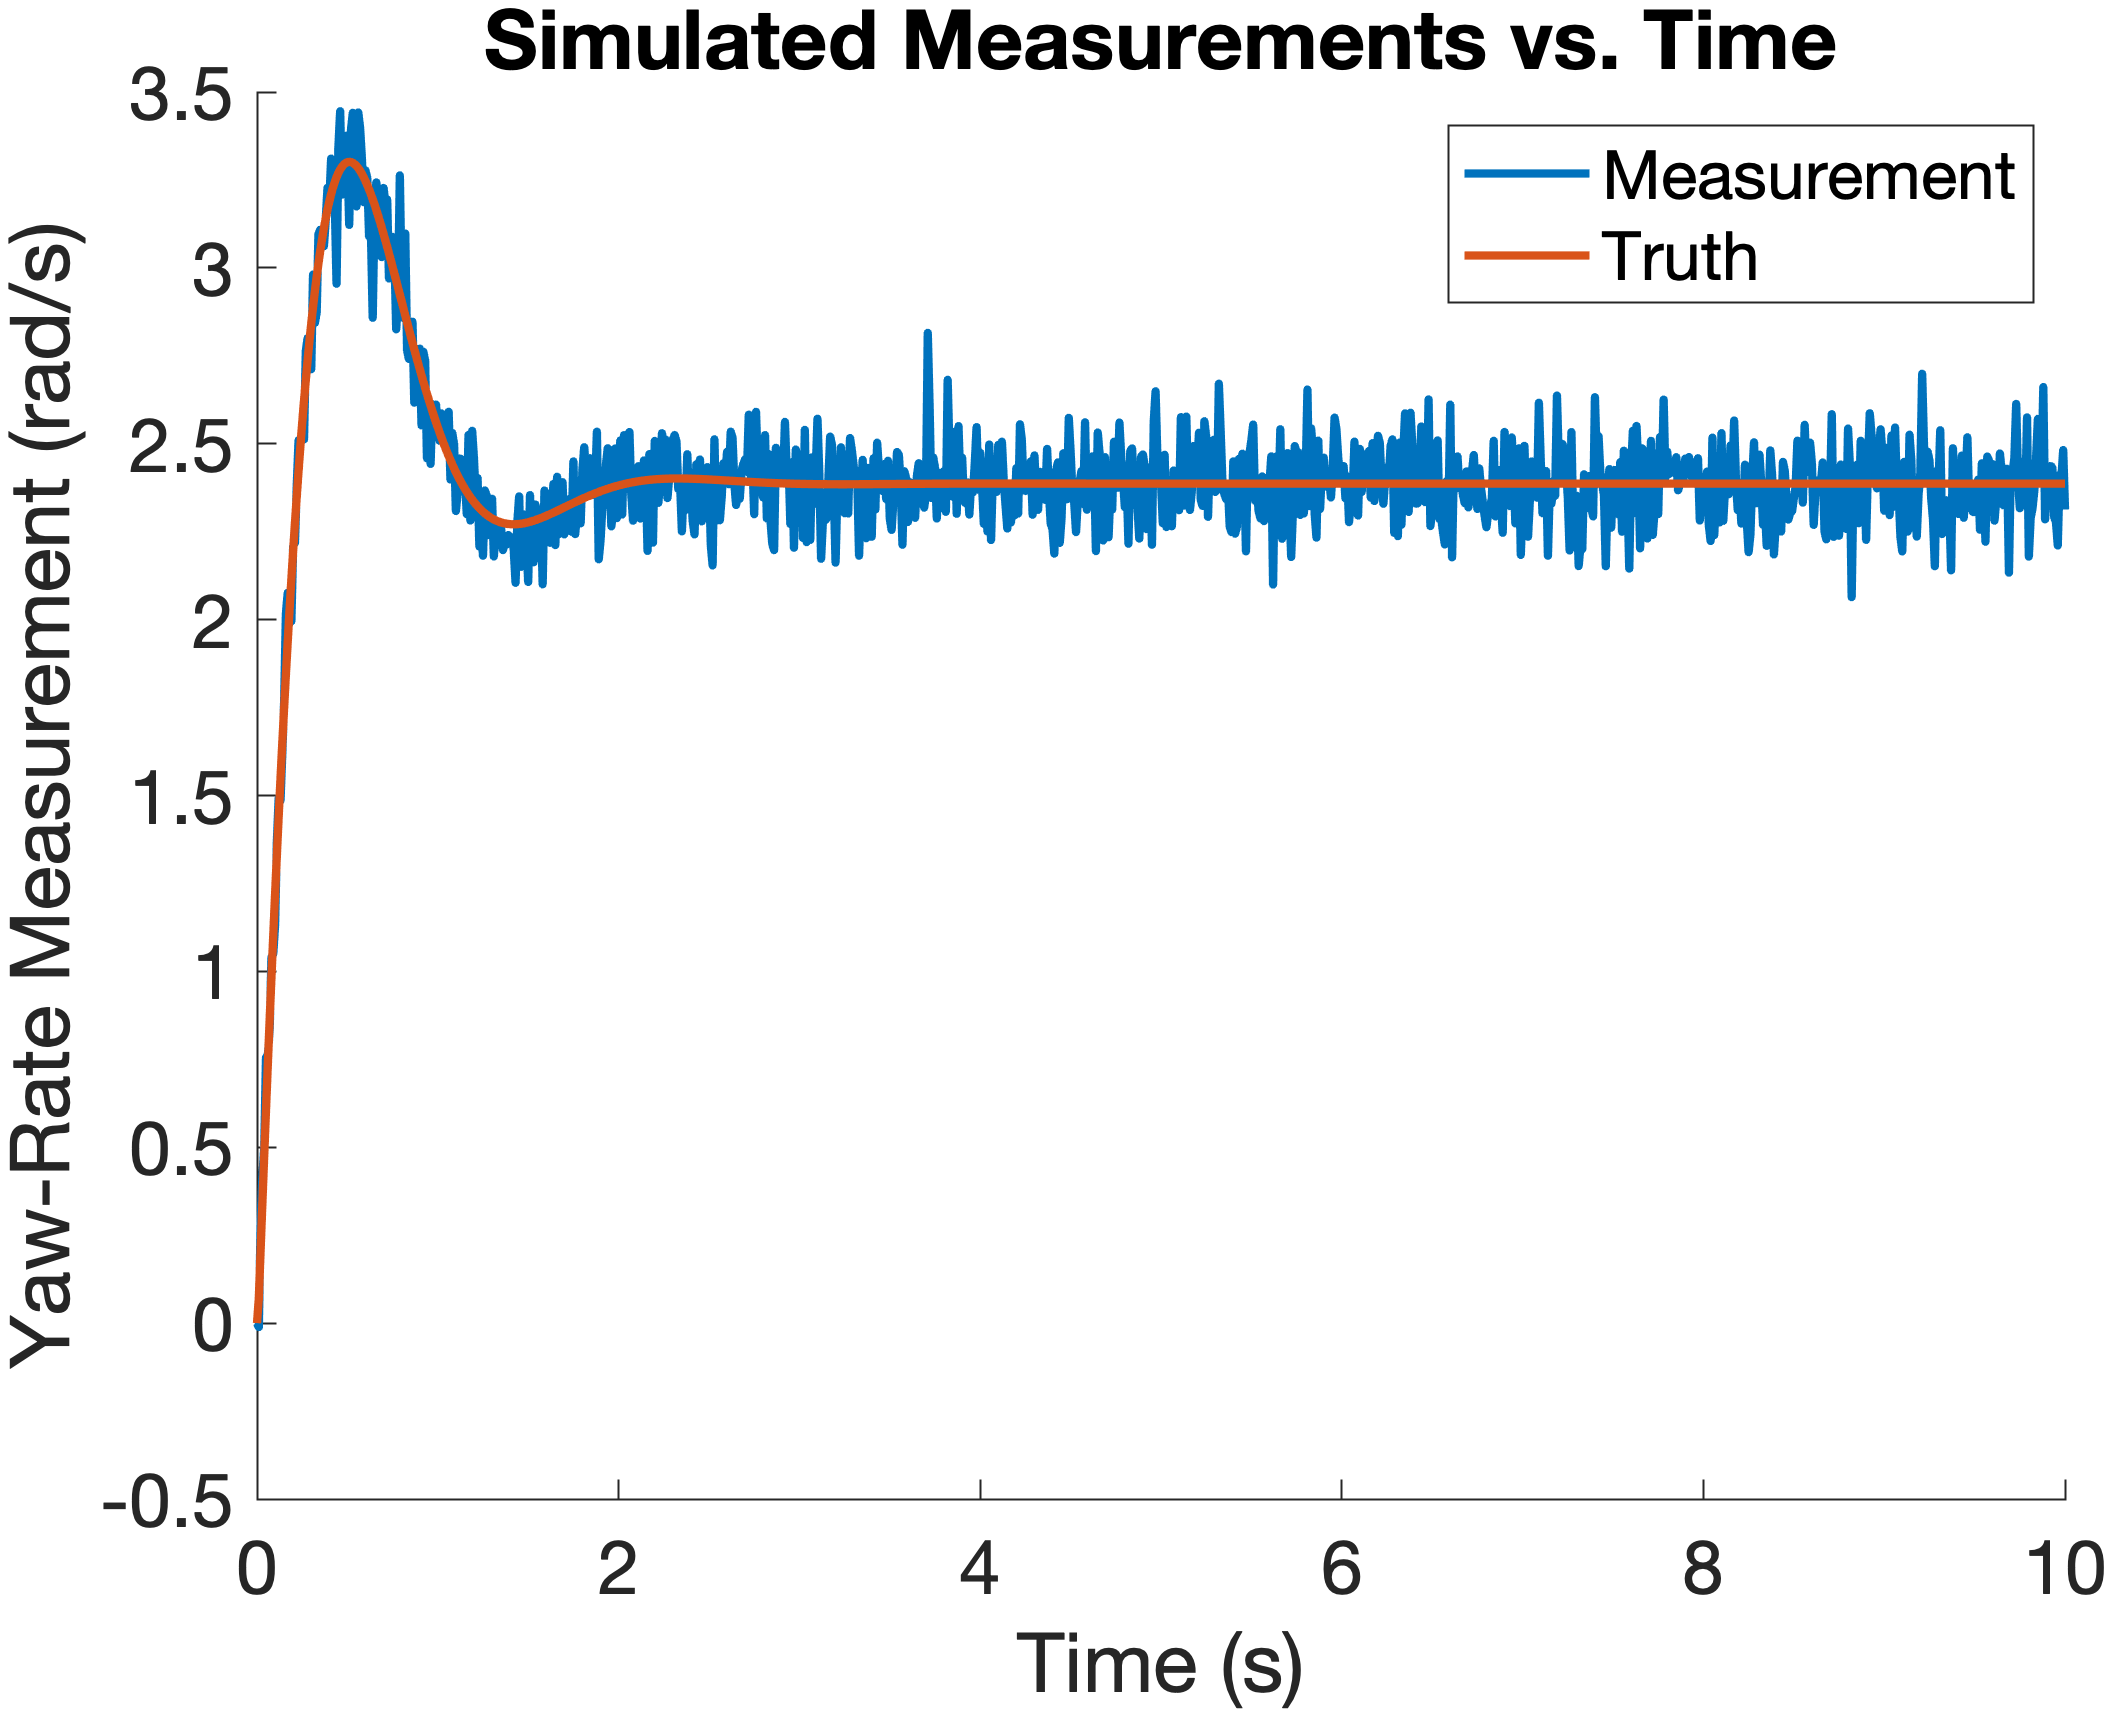
\includegraphics[width=0.75\linewidth]{../figures/p4a_meas.png}
    \caption{Simulated Measurement vs. Time}\label{fig:p4a_meas}
\end{figure}
\begin{figure}[H]
    \centering
    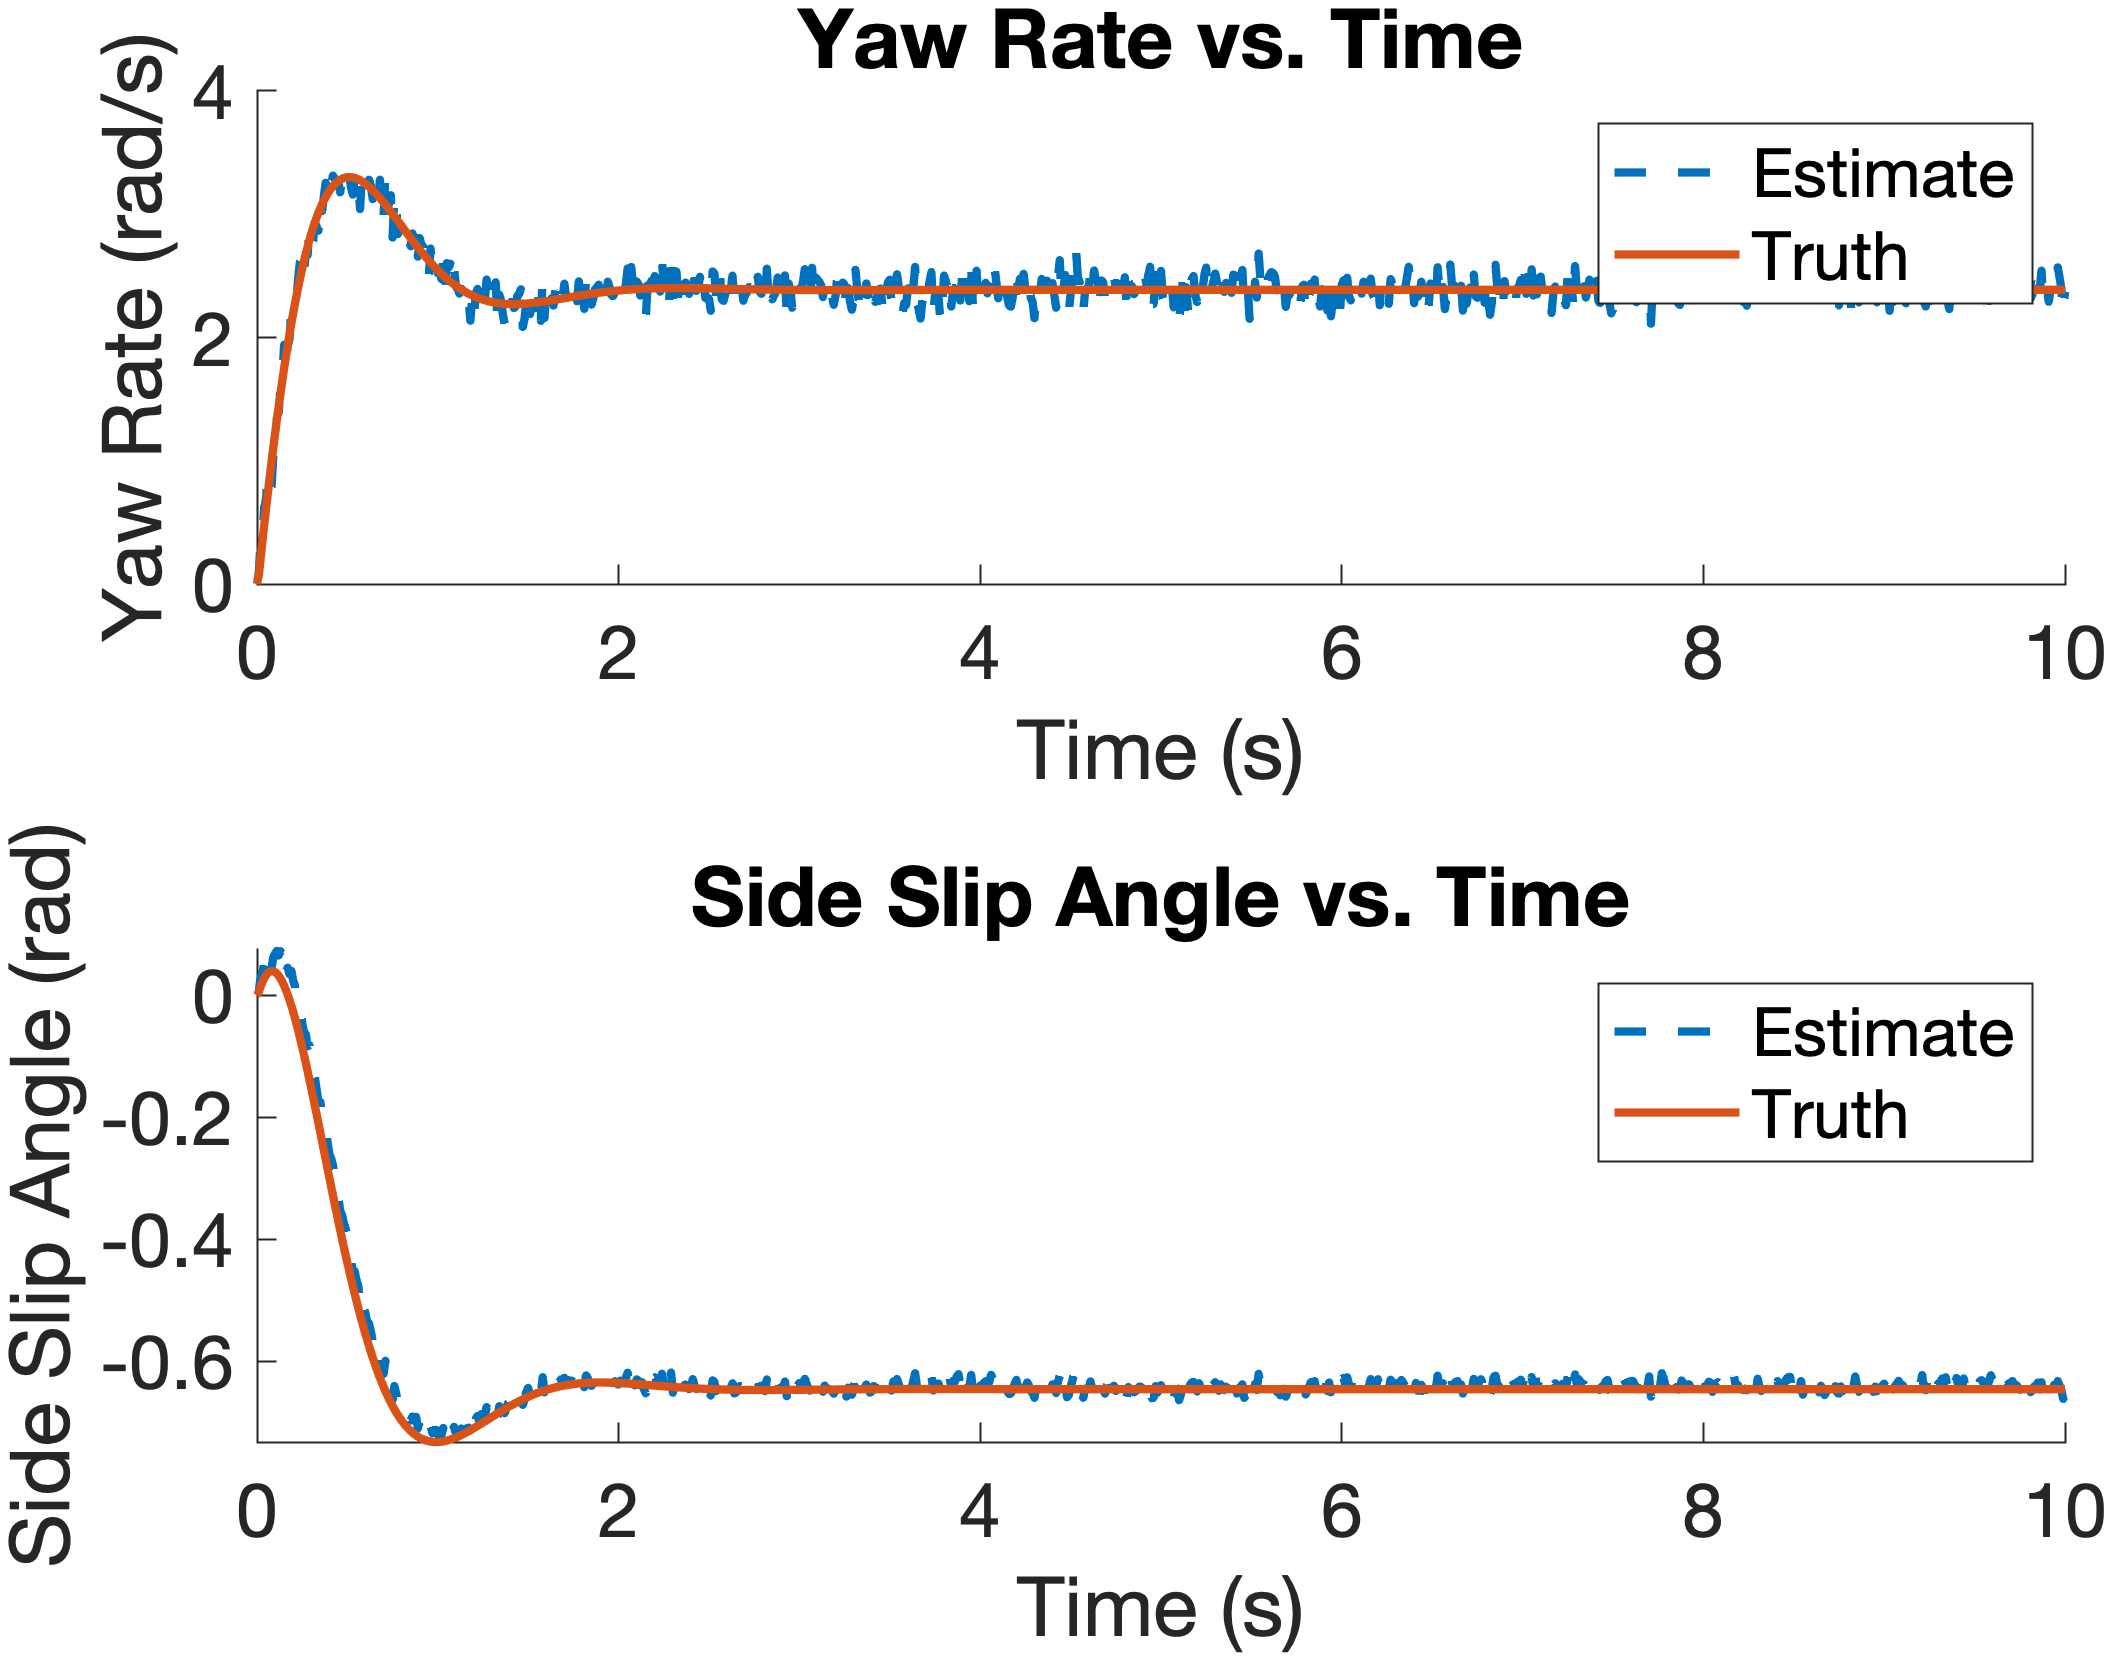
\includegraphics[width=0.75\linewidth]{../figures/p4a_kf.png}
    \caption{State Estimates \& Truth vs. Time}\label{fig:p4a_kf}
\end{figure}
The yaw-rate is estimated fairly well, which is to be expected as we have a direct measurement of the state as well as a model for it.  The side-slip angle estimates well after a significant amount of tuning.  The process noise on that term has to be turned down significantly.  The resulting $Q_d$ is as follows:
\begin{gather*}
    Q_d = \begin{bmatrix}
        1 & 0\\
        0 & 0.03
    \end{bmatrix}
\end{gather*}

\subsection*{Part B}
Now somebody has loaded the trunk of the vehicle with bricks, changing the CG of the vehicle so now the actual model (at 25 m/s) is:
\begin{gather}
    \dot{X} = \begin{bmatrix}
        -2.42 &  4 \\
        -0.99 & -2
    \end{bmatrix}\begin{bmatrix}
        \dot{\Psi} \\
        \beta
    \end{bmatrix} + \begin{bmatrix}
        18 \\
        1
    \end{bmatrix}\delta \\
    y_k = \begin{bmatrix}
        1 & 0
    \end{bmatrix}X_k + \nu_k 
\end{gather}
NOTE: We do not know that somebody has loaded the trunk and that the C.G. has changed, therefore we must use the model for part a in our Kalman Filter.\\
Redo part a. Can you estimate the slip angle correctly? Try various $Q_d$.
\subsection*{Solution}
\begin{figure}[H]
    \centering
    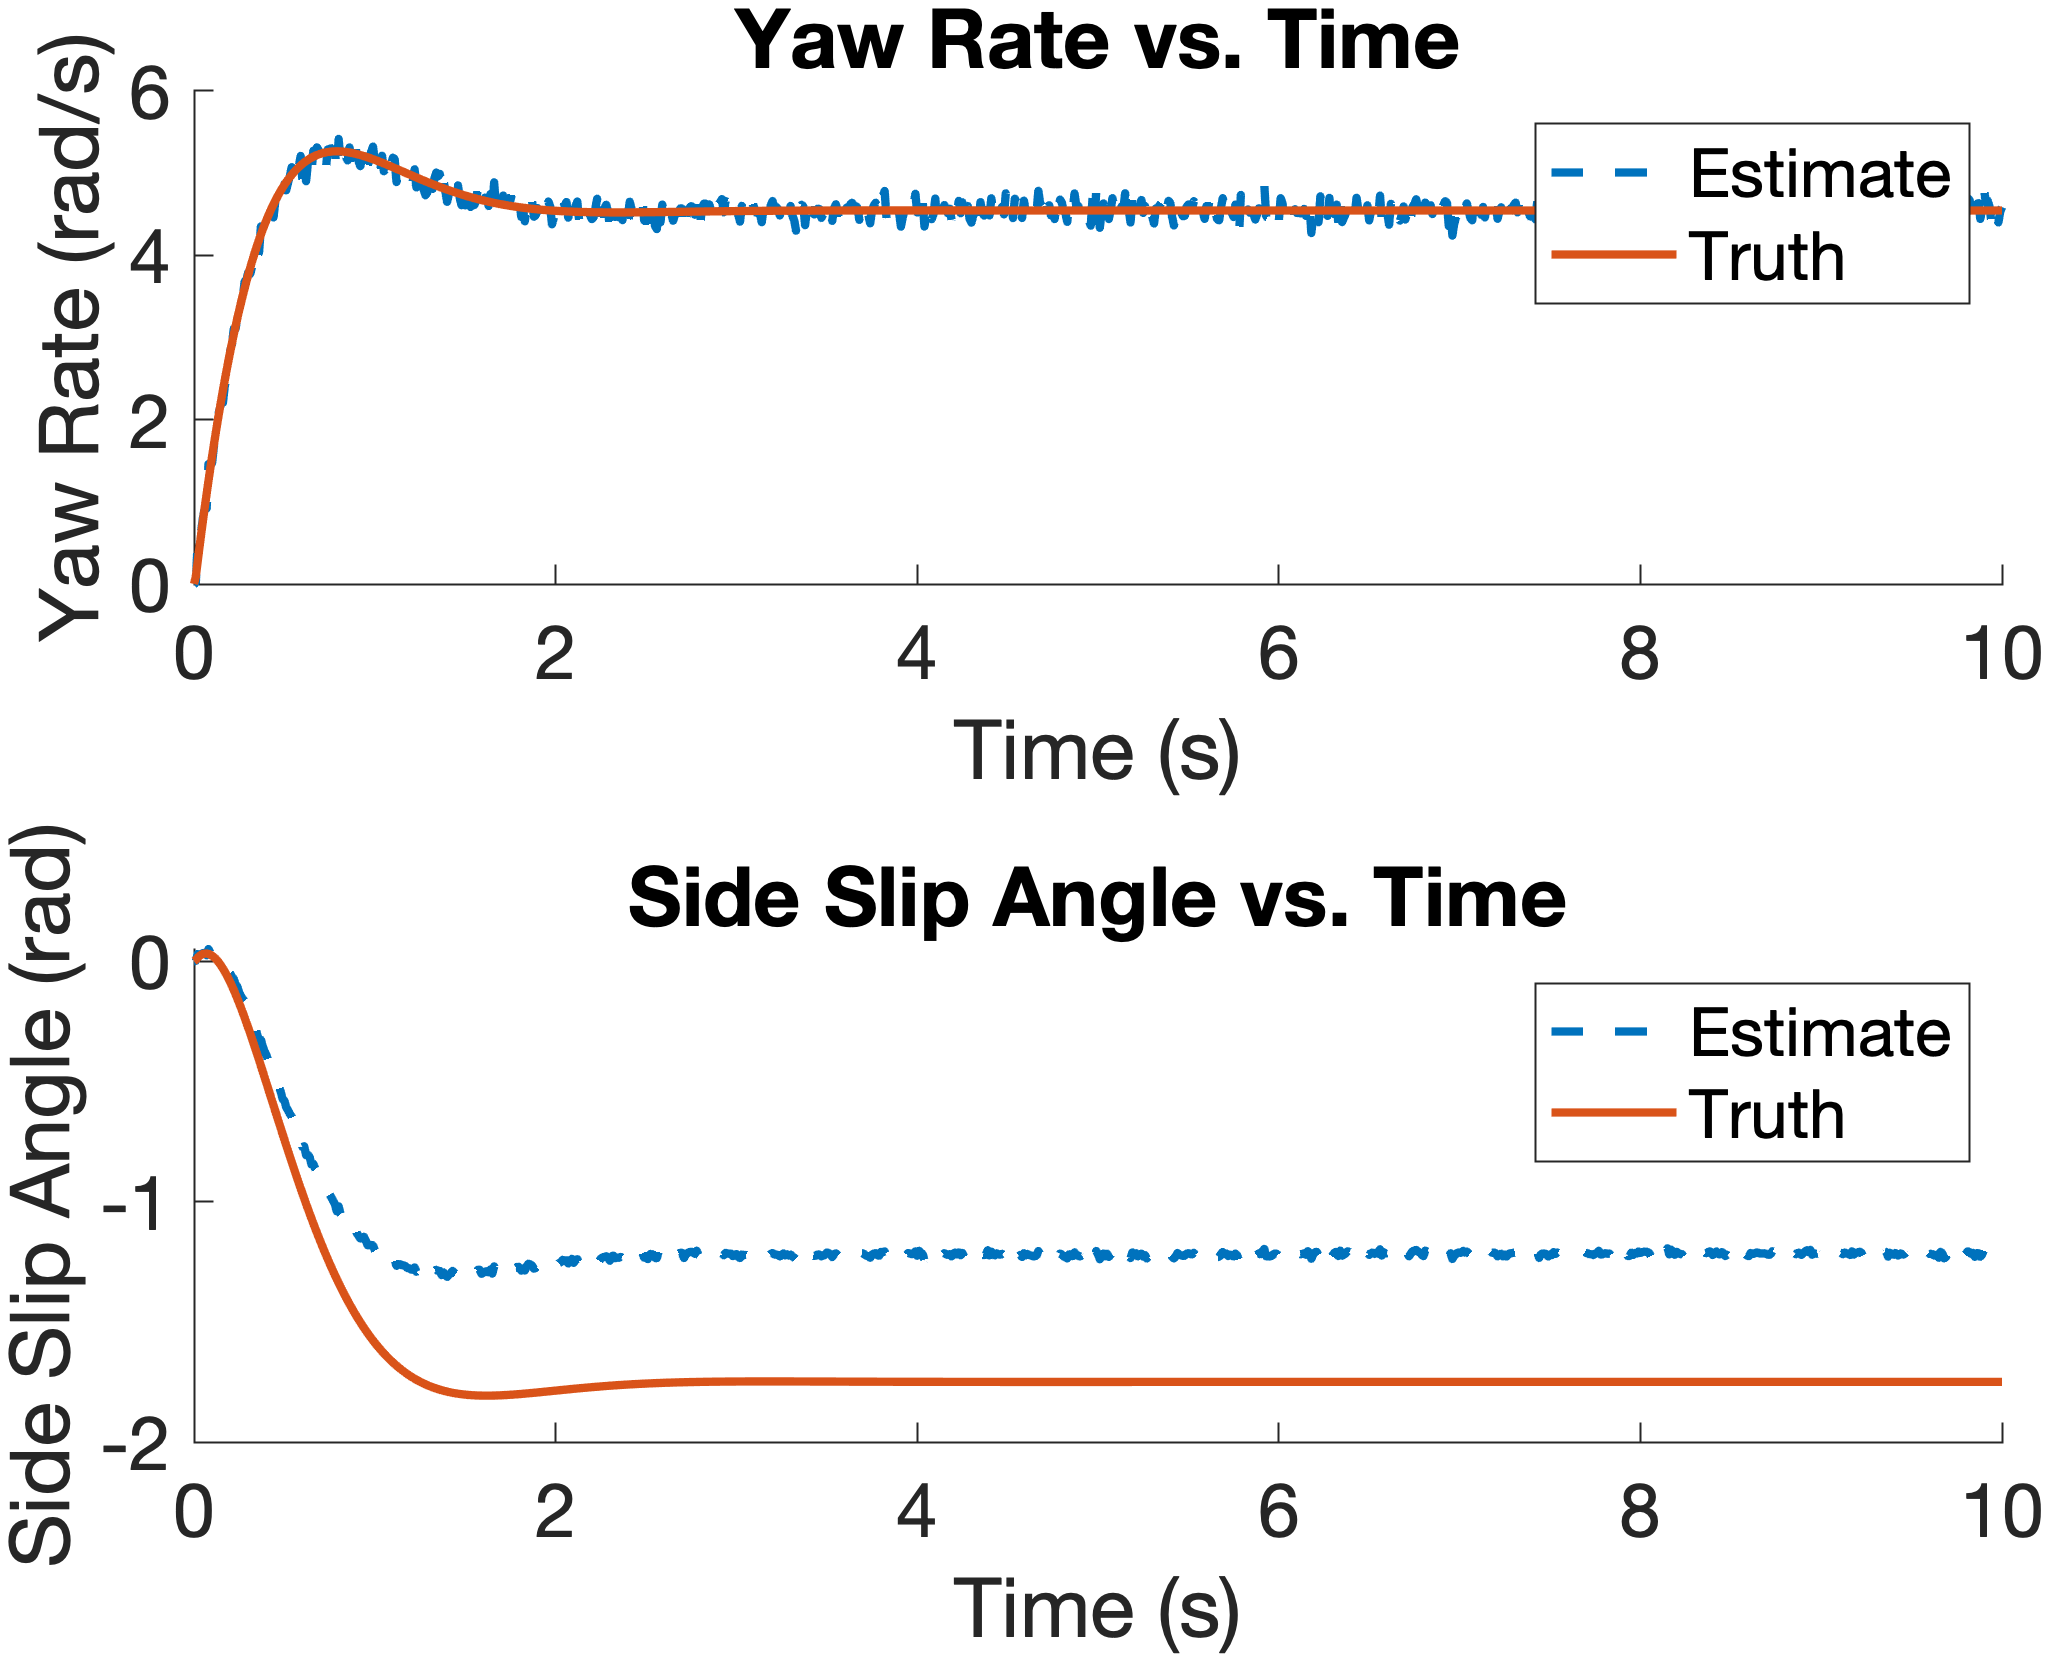
\includegraphics[width=0.75\linewidth]{../figures/p4b_kf.png}
    \caption{State Estimates \& Truth vs. Time}\label{fig:p4b_kf}
\end{figure}
The slip angle can be estimated correctly given that the process noise on the slip angle is double from Part A.  The same was done to the process noise on the yaw-rate.  The resulting $Q_d$ is as follows:
\begin{gather*}
    Q_d = \begin{bmatrix}
        2 & 0\\
        0 & 0.06
    \end{bmatrix}
\end{gather*}

\subsection*{Part C}
Now lets say we have a noisy measurement of the slip angle $(\eta_k\sim N(0,0.5^2))$:
\begin{gather}
    y_k = \begin{bmatrix}
        1 & 0 \\
        0 & 1
    \end{bmatrix}X_k + \begin{bmatrix}
        \nu_k \\
        \eta_k
    \end{bmatrix}
\end{gather}
Assuming the sensor noises are uncorrelated, what is R?
\subsection*{Solution}

\subsection*{Part D}
Redo part a.  What is the effect of changing the element $Q_d$ associated with the slip angle estimate.  What must $Q_d$ equal to ensure an unbiased estimate of the states (How much filtering does that provide)?
\subsection*{Solution}
\begin{figure}[H]
    \centering
    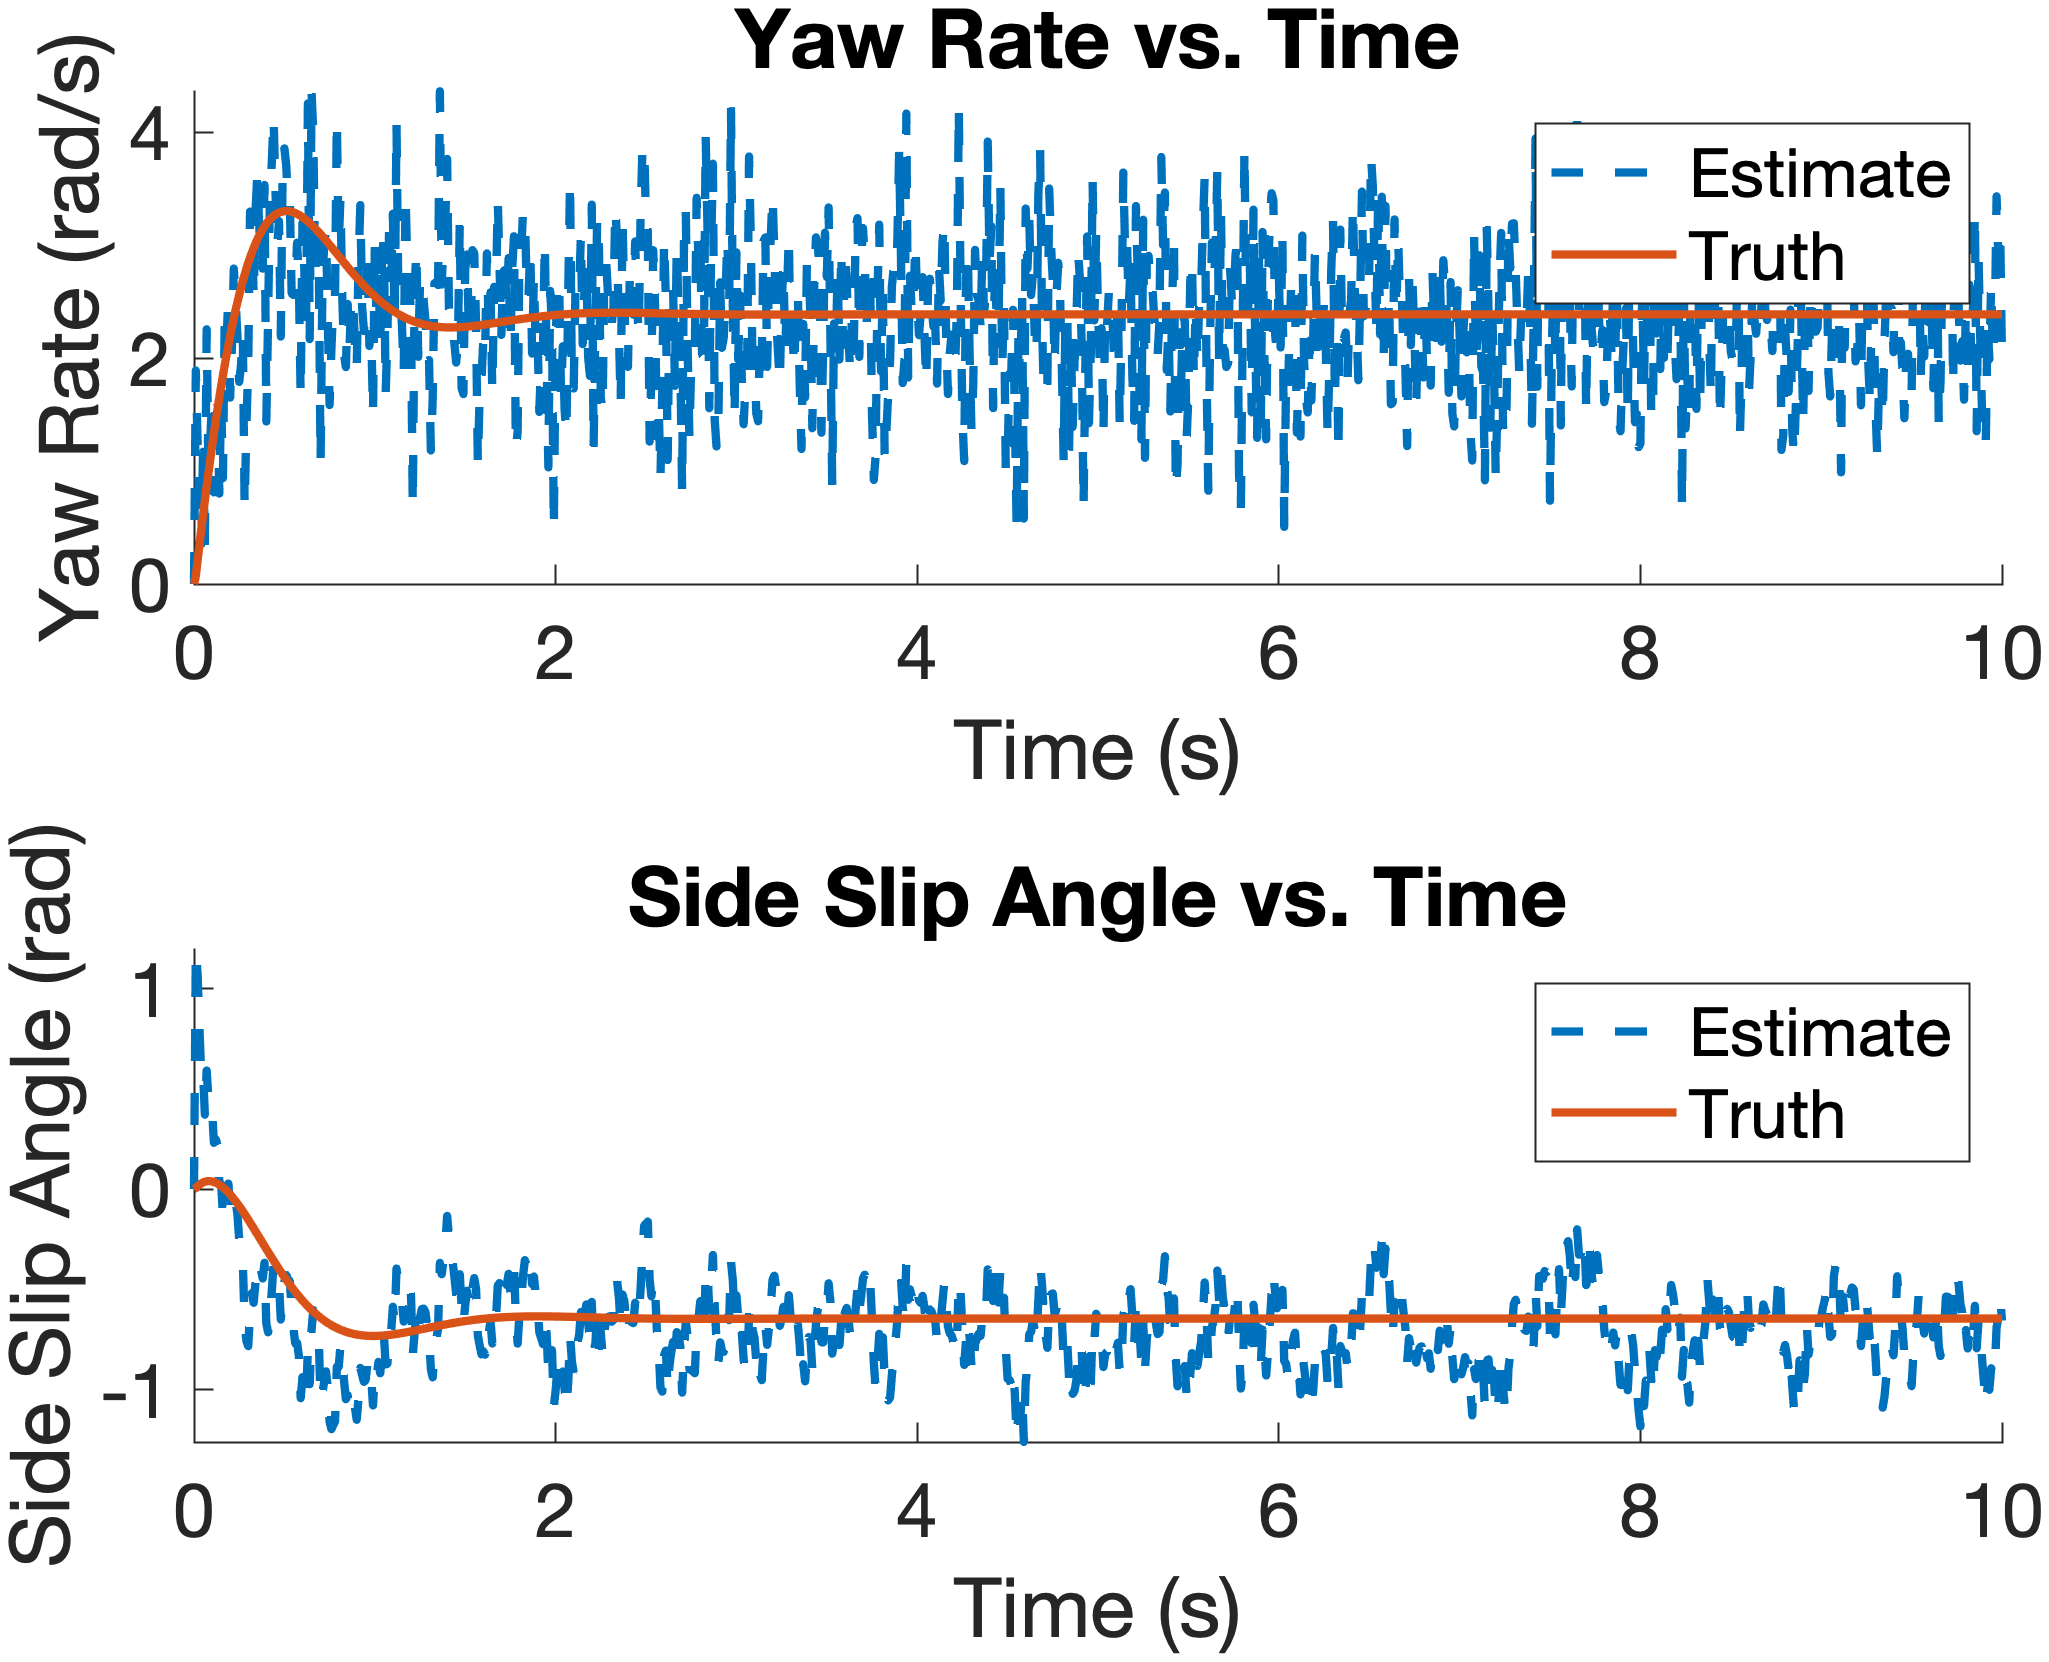
\includegraphics[width=0.75\linewidth]{../figures/p4d_kf.png}
    \caption{State Estimates \& Truth vs. Time}\label{fig:p4d_kf}
\end{figure}
The $Q_d$ calculated to get unbiased state estimates is as follows:
\begin{gather*}
    Q_d = \begin{bmatrix}
        2 & 0\\
        0 & 0.02
    \end{bmatrix}
\end{gather*}
The SNR between the true state and the measurement is $\sim -3.9476$ while the SNR between the measurement between the esitmate is $\sim 2.7786$.  Clearly there is a fair bit of filtering being done by the Kalman Filter.  Compared to the other two filters, the estimate is much noisier, but the trust is more evenly split between the measurement and process model.

\section*{Appendix A: Part I Code}
\lstinputlisting[
frame=single,
numbers=left,
style=Matlab-bw
]{../matlab/p1.m}

\section*{Appendix B: Part II Code}
\lstinputlisting[
frame=single,
numbers=left,
style=Matlab-bw
]{../matlab/p2.m}

\section*{Appendix C: Part III Code}
\lstinputlisting[
frame=single,
numbers=left,
style=Matlab-bw
]{../matlab/p3.m}

\section*{Appendix D: Part IV Code}
\lstinputlisting[
frame=single,
numbers=left,
style=Matlab-bw
]{../matlab/p4.m}

\end{document}
